\documentclass{foi}

\usepackage[document]{ragged2e}

\vrstaRada{\zavrsni} % \diplomski
\title{Prilagodljiv sustav za smanjenje svjetlosnog zasljepljivanja vozača}

\author{Stjepan Petrović}
\spolStudenta{\musko} % \zensko ili \musko
\mentor{Boris Tomaš}
\spolMentora{\musko} % \zensko ili \musko
\godina{2023}
\mjesec{rujan}
\date{2023}
\status{redoviti}
\indeks{0016150314}
\smjer{Informacijski i poslovni sustavi} % (ili Poslovni sustavi, Ekonomika poduzetništva, Primjena informacijske tehnologije u poslovanju, Informacijsko i programsko inženjerstvo, Baze podataka i baze znanja, Organizacija poslovnih sustava, Informatika u obrazovanju)
\titulaProfesora{Doc. dr. sc.}

\sazetak{Tema rada je izrada prilagodljivog sustava za smanjenje svjetlosnog zasljepljivanja vozača što predstavlja fizički prototip koji čini LCD matrica, dvije web kamere i laptop kao procesna jedinica. Svjetlosno zasljepljivanje kod vozača uzrokuje pojavu Troxlerovog efekta koji uzrokuje trenutnu sljepoću zbog čega se povečava vozačevo vrijeme za reakciju. U radu su opisani postojeći sustavi protiv zasljepljivanja od kojih su pojedini tek izumi opisani u patentima, a pojedini su realizirani kao prototipi ili proizvodi spremni za tržište. Izazov je bio spojiti četiri komponente (komponentu za pozicioniranje očiju vozača, komponentu za pozicioniranje zasljepljujućeg svjetla, komponentu za zaštitu od zasljepljujućeg svjetla i komponentu procesne jedinice i hardver), od kojih svaka ima svoju važnost i način pristupa, u jedan funkcionalan sustav čiji je prototip realiziran u ovome radu i koji odgovara na pitanje: kako preko kamera prepoznati izvor zasljepljujućeg svjetla i zaštiti oči vozača na način da se preko LCD matrice spriječi prolazak zasljepljujućeg svjetla do očiju vozača. Kako bi se izradio odgovarajući sustav korištena je biblioteka OpenCV (engl. \emph{Open Source Computer Vision Library}) koja je kao projekt pokrenuta od strane Intel korporacije, a pruža softver za strojno učenje i računalni vid u realnom vremenu i korišten je programski jezik Python. Programski kod i \LaTeX \space dokumentacija ovog rada je verzionizirana na GitHub repozitoriju, kojem se može pristupiti preko poveznice: \url{https://github.com/StjepanPetrovic/Prilagodljiv-sustav-za-smanjenje-svjetlosnog-zasljepljivanja-vozaca}.}

\kljucneRijeci{računalni vid; OpenCV; vozilo; zasljepljivanje; Troxlerov efekt; LCD; Python; kamera;}

%\renewcommand*{\lstlistlistingname}{Popis programskih kodova}

\begin{document}

\justifying

\counterwithout{lstlisting}{chapter}

\captionsetup[lstlisting]{font={small, sf},labelfont={sf, small}}

\maketitle

\tableofcontents

\pagestyle{plain}
\chapter{Uvod}

Ovim završnim radom obrađeni su teorijski koncepti na kojima se temelji rad, istražena je literatura odnosno istraženi su postojeći sustavi, opisan je tijek izrade i konačan rezultat izrade \textbf{prilagodljivog sustava za smanjenje svjetlosnog zasljepljivanja vozača} te je provedeno testiranje sustava.

U nastavku rada za izraz „prilagodljiv sustav za smanjenje svjetlosnog zasljepljivanja vozača" koristit će se skraćena inačica „\textbf{sustav}“.

\flushleft U uvodu je:
\justifying
\begin{itemize}[noitemsep]
    \item opisan problem koji ovaj rad pokušava riješiti,
    \item naveden je cilj rada koji opisuje na koji način će biti prototip realiziran,
    \item navedena je motivacija autora za izradu ovog rada,
    \item opisane su metode i tehnike rada koje su se koristile prilikom izrade rada.
\end{itemize}

\flushleft Nakon čitanja poglavlja "Pregled literature" steći će se bolje razumijevanje sustava koji se opisuje u ovom radu, a u njemu je opisano trenutno stanje tehnologije (engl. \emph{state of the art}) i to:
\justifying
\begin{itemize}[noitemsep]
    \item opisan je fenomen Troxlerov efekt koji se javlja prilikom svjetlosnog zasljepljivanja,
    \item opisani su postojeći sustavi koji su već ostvareni kao proizvodi na tržištu ili su tek opisani kroz patent ili prototip.
\end{itemize}

U poglavlju "Izrada sustava" opisan je tijek izrade sustava, koji je popraćen s teorijskim konceptima, kroz opis pojedinih komponenata sustava te je opisan tijek testiranja sustava i opisani su rezultati testiranja.

Na kraju rada je zaključak kojim su protumačeni rezultati izrade i testiranja sustava, navedeni su prijedlozi za buduća usavršavanja sustava i navedeni su zaključni dojmovi autora.

\section{Definicija problema}

 Potrebno je napraviti sustav koji u realnom vremenu prepoznaje izvor zasljepljujućeg svjetla te reagira na način da polarizira određeni dio reaktivne komponente (LCD matrice) koja bi se nalazila na vjetrobranskom staklu vozila te na taj način smanji jačinu zasljepljujućeg svjetla ispred vozača u vozilu.

 Problem se temelji na potrebi za smanjenjem zasljepljujućeg svjetla koje može uzrokovati privremeno zaslijepljenje vozača, kao što su svjetla iz suprotnog smjera tijekom noći ili sunčeva svjetlost tijekom dana. Cilj ove tehnologije je selektivno smanjiti intenzitet zasljepljujućeg svjetla putem transparentne površine odnosno reaktivne komponente koja ima sposobnost kontroliranja transparentnosti na određenim mjestima na površini. Budući da je položaj zasljepljujućeg svjetla u okolini mobilan kao i mjesto zatamnjivanja na transparentnoj površini, koriste se algoritmi za identifikaciju položaja zasljepljujućeg svjetla unutar vidnog polja i kalkulacije za izračun mjesta zatamnjivanja.

Uz dodatna ulaganja i razvoj, ovaj prototip može postati vrlo popularan i koristan proizvod svakom vozaču u vozilu jer će pružiti zaštitu u noćnoj vožnji od zasljepljujuće svjetlosti, koja usmjerena u oči vozača za vrlo kratak trenutak može ugroziti vozača. Najčešće su izvor te svjetlosti duga svjetla na vozilu vozača koji zbog neopreznosti ne isključi duga svjetla u trenutku kada dolazi ususret drugom vozilu čiji će vozač zbog toga biti svjetlosno zasljepljen te na trenutak neće moći vidjeti kuda vozi što može loše utjecati na vozača. Zato je potrebno napraviti sustav koji će:
\begin{itemize}[noitemsep]
    \item prepoznati i pozicionirati izvor svjetla te oči vozača koristeći kamere,
    \item kalibrirati komponente i uspješno ih povezati u jedan cjelovit funkcionalan sustav.
\end{itemize}

\section{Cilj}

Cilj ovog rada je napraviti prototip koji će moći raditi u stvarnoj okolini, a ta okolina je pojednostavljeno predstavljena u trodimenzionalnom koordinatnom sustavu kao na slici \ref{fig:prikaz_sustava_1}. Za ulazne uređaje pomoću kojih će vidjeti što se događa u okolini vozača će biti uzete dvije web kamere čiji je sadržaj onoga što vide predstavljen kao narančasti i zeleni okvir na slici \ref{fig:prikaz_sustava_1}, a taj sadržaj će obrađivati istrenirani modeli za računalni vid iz biblioteke OpenCV te će tako procesna jedinica znati gdje se nalaze oči vozača i izvor svjetla koji su predstavljeni kao crveni krugovi odnosno baze valjka na narančastom i zelenom okviru na slici \ref{fig:prikaz_sustava_1}. Kada procesna jedinica to zna, potrebno će biti pomoću algoritma izračunati koji točno dio LCD matrice treba polarizirati/zatamniti, a taj dio koji treba polarizirati je prikazan na slici \ref{fig:prikaz_sustava_1} kao crveni krug na crnom okviru odnosno intersekcija žutog plašta valjka, koji predstavlja svjetlost, sa crnim okvirom koji predstavlja reaktivnu komponentu (LCD matricu). Interaktivnom grafu sa slike \ref{fig:prikaz_sustava_1} može se pristupiti preko linka: \url{https://www.geogebra.org/m/hvzfyjfz}.

\begin{figure}[h!]
    \centering
    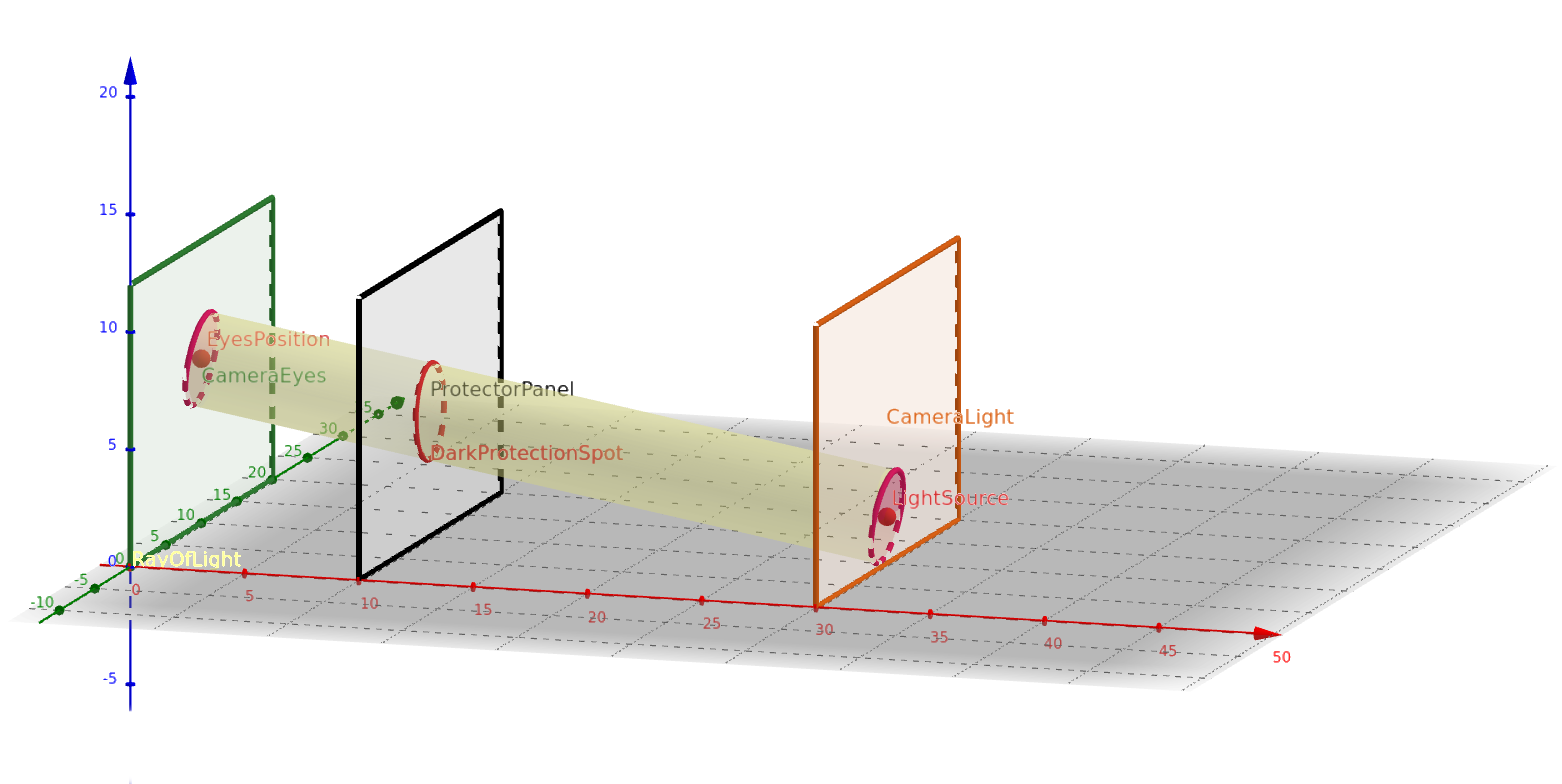
\includegraphics[width=0.9\textwidth]{slike/graf_uvod}
    \captionsetup{font={small}}
    \caption{Pojednostavljen prikaz sustava u trodimenzionalnom koordinatnom sustavu [autorski rad]}
    \label{fig:prikaz_sustava_1}
\end{figure}

Razlog zbog čega će biti uzeta LCD matrica kao reaktivna komponenta koja će sprječavati zasljepljujuće svjetlo da dođe do očiju vozača je taj što može biti prozirna i moguće je gledati kroz nju, zbog čega neće smetati na vjetrobranskom staklu prilikom vožnje, a lako ju je moguće napraviti neprozirnom na način da se zaslon polarizira odnosno da se pikseli postave na crnu boju.

\begin{flushleft}Sustav protiv zasljepljivanja će se sastojati od četiri komponente koje će biti u radu obrađene:\end{flushleft}
\begin{itemize}[noitemsep]
    \item Procesna jedinica (laptop) i hardver (web kamere i LCD matrica),
    \item Komponenta za prepoznavanje i pozicioniranje izvora svjetla,
    \item Komponenta za prepoznavanje i pozicioniranje očiju vozača,
    \item Komponenta za polarizaciju LCD matrice kao reaktivne komponente.
\end{itemize}

\section{Motivacija za rad}

Motivacija za odabir ove teme je bila misao da će se autor okušati u stvaranju sustava protiv zasljepljivanja vlasnika automobila za kojeg i u modernoj automobilskoj industriji još ne postoji izrađeno rješenje koje je optimalno za korištenje u realnim uvjetima – zbog čega je gore i rečeno da bi uz daljnja ulaganja i razvoj,  fizički prototip koji je izrađen u svrhu ovog završnog rada mogao biti popularan. Postoji velik broj raspisanih patenata od strane najkonkurentnijih svjetskih proizvođača (General Motors \cite{Bogdan2023}, Bosch \cite{Chris}, Ford \cite{ElectronicSpecifier2016}, Apple \cite{OwenMal2018}) što ostavlja dojam da će skorija budućnost biti jako dinamična utrka za osvajanje tržišta proizvodom koji će, osim borbe sa svjetlosnim zasljepljenjem, donijeti i dodatne mogućnosti kao što je uvođenje proširene stvarnosti (engl. \emph{Augmented Reality - AR}) na vjetrobransko staklo \cite{Bogdan2023} \cite{Ungureanu2020}.

Velik broj nesreća, od 12\% do 15\% nesreća koje se dogode noći na američkim cestama su prouzrokovane svjetlosnim zasljepljenjem vozača \cite{Hu2022}, a još veći je broj vozila koji se svakim danom povećava na prometnicama širom svijeta \cite{LeasingOptions2021}, stoga moderna automobilska industrija sve više pokušava proizvesti automobile koji će imati ugrađen takav sustav za zaštitu vozača – što donosi velik značaj ovoj temi te poticaj za daljnje istraživanje i razvoj proizvoda koji će spriječiti povećanje broja prometnih nesreća prouzrokovanih svjetlosnim zasljepljenjem vozača.

\section{Metode i tehnike rada}

Tijekom razrade teme korišteni su izvori s interneta kao što su istraživački radovi, članci, blogovi, patenti (\href{https://patents.google.com/}{Google Patents}) te službena dokumentacija programskog jezika Python i biblioteke OpenCV. Programski kod odnosno programsko rješenje je djelo autora rada.

U alatima GeoGebra i draw.io su izrađeni pojednostavljeni prikazi sustava zbog lakšeg razumijevanja. Podijeljeni su i linkovi na videozapise koji prikazuju kako sustav radi.

Programski kod i \LaTeX \space dokumentacija je verzionizirana na GitHub repozitoriju, kojem se može pristupiti preko poveznice: \url{https://github.com/StjepanPetrovic/Prilagodljiv-sustav-za-smanjenje-svjetlosnog-zasljepljivanja-vozaca}.

\chapter{Pregled literature}

U nastavku ovog poglavlja obrađuje se literatura koja je vezana za temu sustava za smanjenje svjetlosnog zasljepljivanja vozača.

\section{Troxlerov efekt}

Razlog zbog kojeg je potreban ovakav sustav je Troxlerov efekt (engl. \emph{Troxler Effect} ili \emph{fading effect}) koji može nastati tijekom vožnje \cite{Autoevolution2022}. Troxlerov efekt je poznat fenomen u području percepcije i vizualne psihologije. Ovaj efekt opisuje trenutnu sljepoću i ilustrira kako naš mozak percipira i procesira vizualne informacije te kako se te informacije mogu mijenjati ako gledamo na istu stvar dulje vrijeme ili ako smo pod utjecajem jakog izvora svjetlosti zbog čega se povečava vozačevo vrijeme za reakciju \cite[str. 208]{P2014}.

Osnovna pojava Troxlerovog efekta događa se kada fiksiramo svoj pogled na jedan objekt ili točku na nekom statičkom pozadinom duže vrijeme. Kako vrijeme prolazi, percepcija tog objekta ili točke počinje mijenjati. Okolni detalji i boje počinju blijedjeti i nestajati iz našeg vidnog polja \cite[str. 664]{Kanai2003}. Ako bi se 10 do 15 sekundi fokusirao pogled u crvenu točku na slici \ref{fig:troxlerov_efekt}, mogao bi se iskusiti Troxlerov efekt zbog kojeg će se zeleni krug početi gubiti iz perifernog vida.

\begin{figure}[h!]
    \centering
    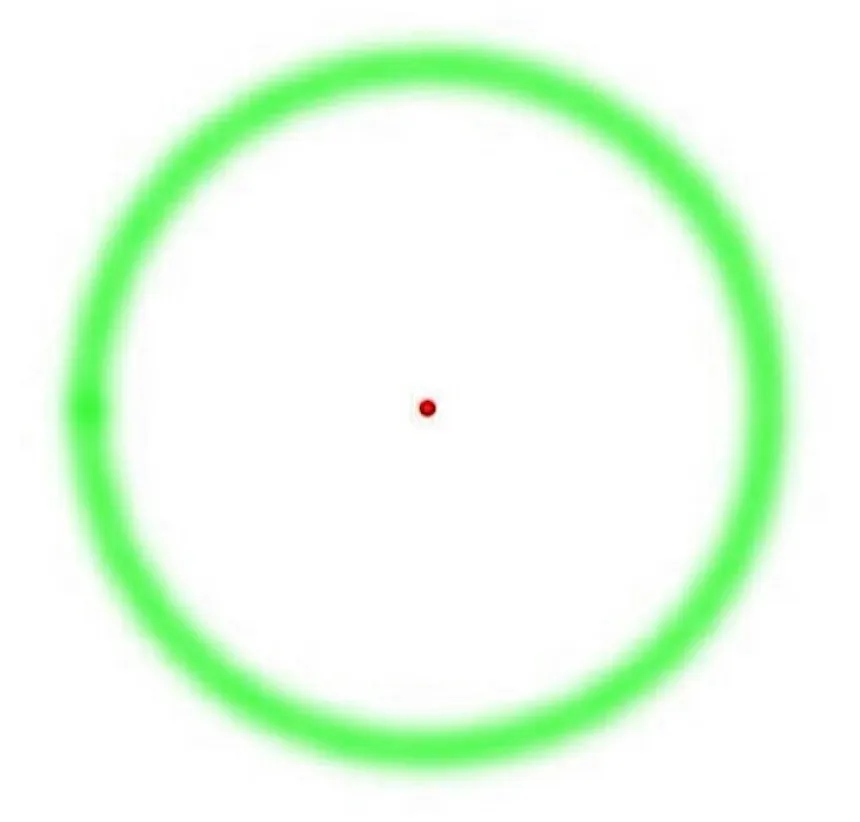
\includegraphics[width=0.7\textwidth]{slike/troxler_effect}
    \captionsetup{font={small}}
    \caption{Prikaz kod kojeg se javlja Troxlerov efekt \cite{Autoevolution2022}}
    \label{fig:troxlerov_efekt}
\end{figure}

\newpage

Zaslijepljivanje je uobičajena situacija u prometu koja se događa kada svjetlosni izvor, kao što su duga svjetla ili sunce, izravno udara u oči vozača. Ovaj nagli prelazak iz tame u svjetlo može uzrokovati privremeno zaslijepljenje vozača. Troxlerov efekt se uklapa u ovu situaciju na način da kada vozač gleda u izvor jakog svjetla, kao što su duga svjetla, to svjetlo postaje dominantno u njihovom vidnom polju. Troxlerov efekt se tada javlja kao rezultat fiksiranja pogleda na tu svijetlu točku. Okolni detalji na cesti, kao što su prometni znakovi, vozila ili pješaci, postaju manje vidljivi jer mozak počinje "zaboravljati" ili smanjivati percepciju tih podražaja koji se ne mijenjaju. Dakle, vozač može primijetiti da su ti detalji na cesti ili druga vozila postali manje vidljivi ili zamagljeni. \cite{Autoevolution2022}

\section{Sustavi za smanjenje svjetlosnog zasljepljivanja vozača}

U nastavku će biti opisani postojeći sustavi koji se koriste u autoindutstriji ili su tek prototipi te patenti koji opisuju takve sustave koji se bore protiv nastanka Troxlerovog efekta odnosno svjetlosnog zasljepljivanja vozača uzrokovanog jakim izvorima svjetla poput dugih svjetala vozila. Takvi sustavi zastupaju jednu od dvije sljedeće ideje odnosno cilja u autoindustriji kada je u pitanju zaštita vozača od zasljepljujuće svjetlosti:

\begin{itemize}[noitemsep]
    \item napraviti sustav koji će štiti jednog vozača, odnosno onog vozača koji se nalazi u automobilu u kojem je takav sustav i ugrađen,
    \item napraviti sutav koji će štiti ostale vozače od dugih svjetala automobila u kojem je takav sustav ugrađen.
\end{itemize}

Na kraju rada u potpoglavlju "Testiranje sustava" je napisana usporedba sustava koji je izrađen ovim radom sa određenim sustavima koji su opisani u ovom potpoglavlj u nastavku.

\subsection{Sustavi namjenjeni zaštiti jednog vozača}

Ovi sustavi imaju namjeru zaštiti samo vozača koji se nalazi u vozilu u kojem je takav sustav i ugrađen. Njime se analiziraju potencijalne prijetnje prema vozaču vlasniku sustava te shodno prijetnjama sustav se pokušava odbraniti od njih.

\subsubsection{Bosch: LCD vizir podržan umjetnom inteligencijom}

Današnja automobilska industrija neprestano radi na razvoju novih tehnologija kako bi poboljšala sigurnost i udobnost vožnje. Jedan od najnovijih inovativnih proizvoda na tržištu prikazan na slici \ref{fig:bosch_lcd}, Boschov LCD vizir podržan umjetnom inteligencijom, predstavlja značajan korak prema ostvarenju ovih ciljeva. Bosch je kompanija koja je jedna od vodećih svjetskih dobavljača tehnologija i usluga \cite{Bosch}.

\begin{figure}[h!]
    \centering
    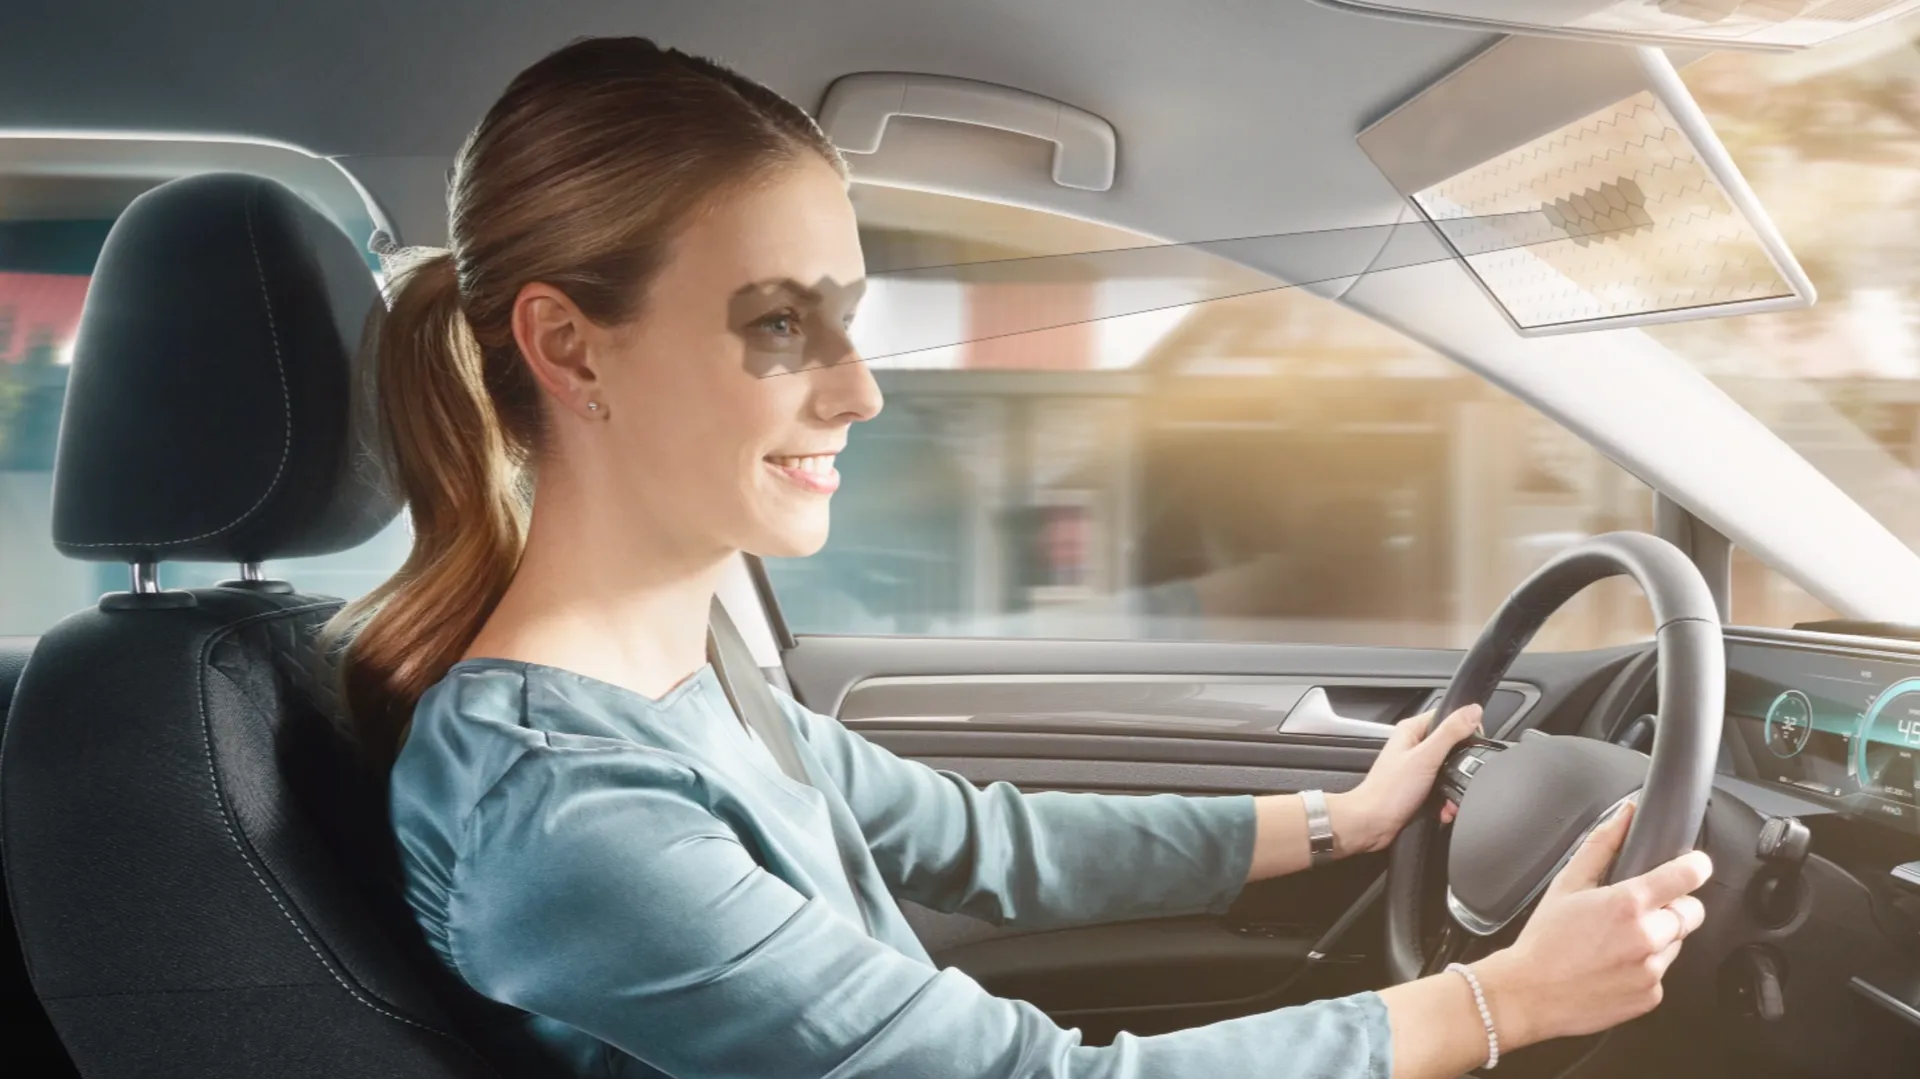
\includegraphics[width=0.6\textwidth]{slike/bosch_virtual_visor}
    \captionsetup{font={small}}
    \caption{Ilustrativni prikaz za Boschov LCD vizir \cite{Chris}}
    \label{fig:bosch_lcd}
\end{figure}

Štitnici za sunce su neizostavan dio svakog vozila već dugi niz godina. Njihova svrha je zaštita vozača i putnika od oštre sunčeve svjetlosti koja može uzrokovati zasljepljivanje i smanjiti vidljivost na cesti. Tradicionalni štitnici za sunce obično su pasivni, što znači da ne reagiraju na promjene uvjeta na cesti. Međutim, Bosch-ova inovacija donosi potpuno novu perspektivu.

Jedna od ključnih značajki Boschovog LCD vizira podržanog umjetnom inteligencijom je njihova sposobnost pametne reakcije na svjetlost. Opremljen je senzorima koji neprestano mjere intenzitet svjetla izvan vozila. Kada senzori otkriju nagli porast svjetlosnog intenziteta, vizir automatski reagira i prigušuju staklo odnosno LCD matricu/panel. Ovo dinamičko prigušivanje omogućuje očuvanje optimalnih uvjeta za vozača i putnike čak i kad se vozi pod jakim sunčevim svjetlom. Njihov vizir, predstavljen na CES 2020, koristi prozirnu LCD matricu i kameru koja se okreće prema vozaču s umjetnom inteligencijom kako bi pratio pogled vozača i blokirao odsjaj svjetlosti \cite{Chris}.

Umjesto tradicionalnog štitnika za sunce koje blokira veliki dio vidnog polja vozača, vizir precizno blokira samo dio vidnog polja gdje se nalazi odsjaj svjetlosti. To omogućuje vozaču da zadrži jasan pogled na cestu i okoliš, dok istovremeno smanjuje ometanje od odsjaja svjetlosti. Vizir koristi napredne algoritme za praćenje lica i očiju kako bi odredio položaj očiju vozača i kut gledanja. Zatim koristi tu informaciju kako bi precizno blokirao odsjaj svjetlosti pomoću prozirnog LCD panela. Panel se može prilagoditi u stvarnom vremenu kako bi osigurao optimalnu vidljivost za vozača.

Ovaj proizvod je tek prototip (slika \ref{fig:bosch_lcd_2}) koji je najsličiniji prototipu koji će biti opisan u ovom radu te ova tehnologija ima potencijal da poboljša sigurnost na cestama smanjenjem rizika od privremenog sljepila uzrokovanog odsjajem svjetlosti. Također može poboljšati udobnost vožnje tako što omogućuje vozačima da zadrže jasan pogled na cestu bez potrebe za neprestanim podešavanjem štitnika za sunce. Bosch nastavlja razvijati Virtual Visor i istraživati nove načine primjene ove tehnologije. U budućnosti bismo mogli vidjeti još naprednije sustave koji koriste umjetnu inteligenciju i strojno učenje kako bi poboljšali sigurnost i udobnost vožnje \cite{Chris}.

Sličan prototip je opisan i u istraživačkom radu "Adaptive LCD Windshield Glare Elimination System" \cite{Shreesha2019} i u radu "Automatic anti-glare system for night time driving using liquid crystal screens" \cite{Pankaj}.

\begin{figure}[h!]
    \centering
    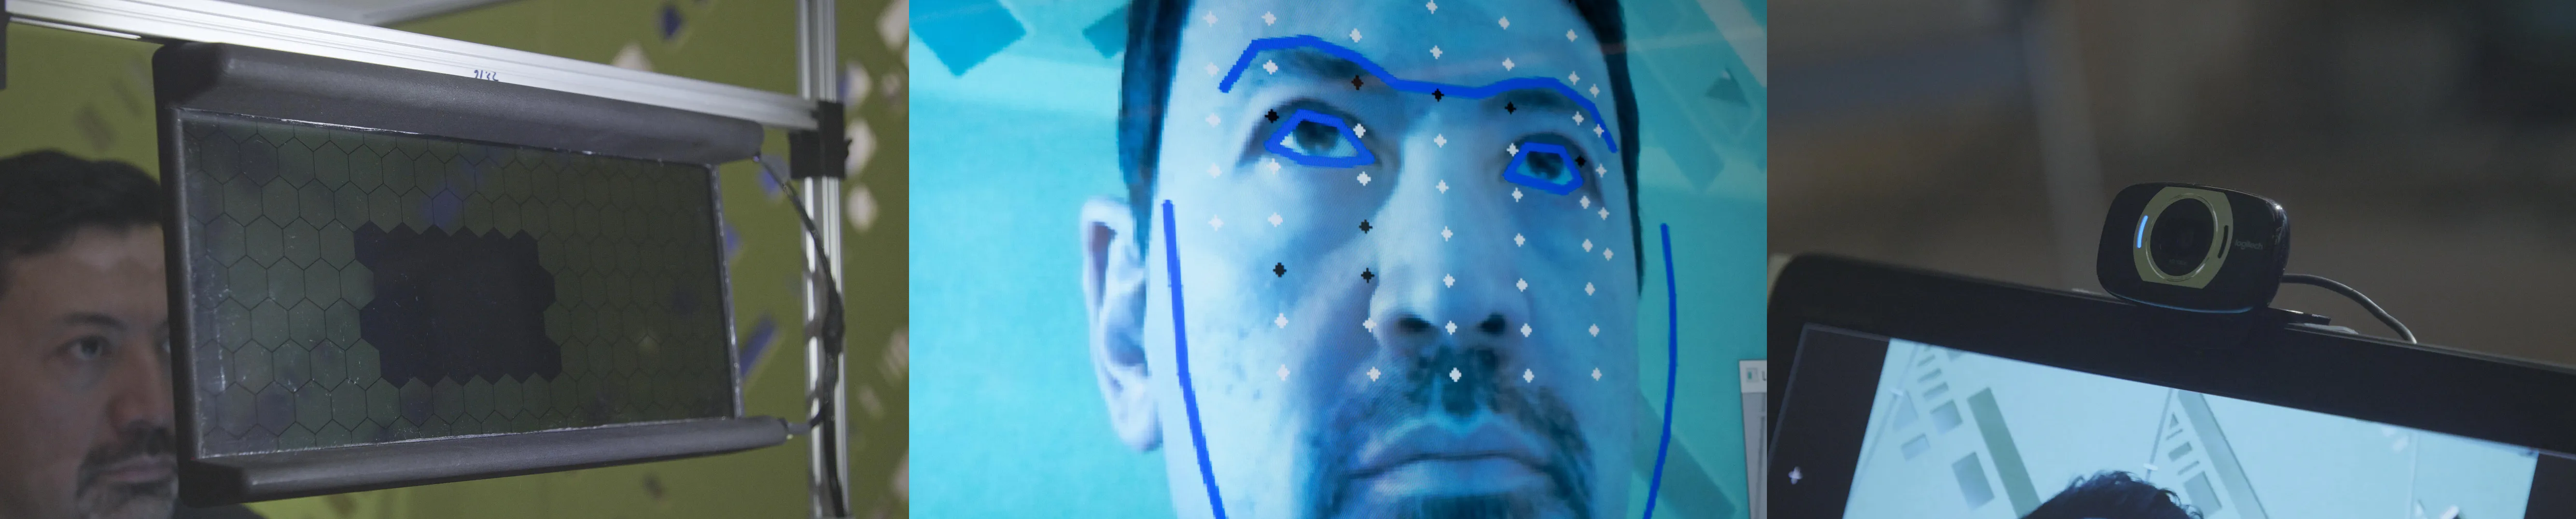
\includegraphics[width=1\textwidth]{slike/bosch-virtual-visor-2}
    \captionsetup{font={small}}
    \caption{Prikaz prototipa za Bosch LCD vizir \cite{Chris}}
    \label{fig:bosch_lcd_2}
\end{figure}

\subsubsection{Patent US2006140502A1: Aktivni vizir}

Ovaj patent napisan je kako bi se riješio problem zasljepljujućeg svjetla koje vozači doživljavaju tijekom vožnje. Zasljepljujuće svjetlo može potjecati od različitih izvora, uključujući svjetla iz suprotnog smjera, sunčevu svjetlost i reflektirajuće površine. Ovaj izum pruža rješenje za automatsko i selektivno smanjenje intenziteta takvog svjetla kako bi vozači zadržali jasnu vidljivost i smanjili rizik od zaslijepljenosti \cite{Allan2006}. Skica izuma prikazana je na slici \ref{fig:patent1}.

\begin{figure}[h!]
    \centering
    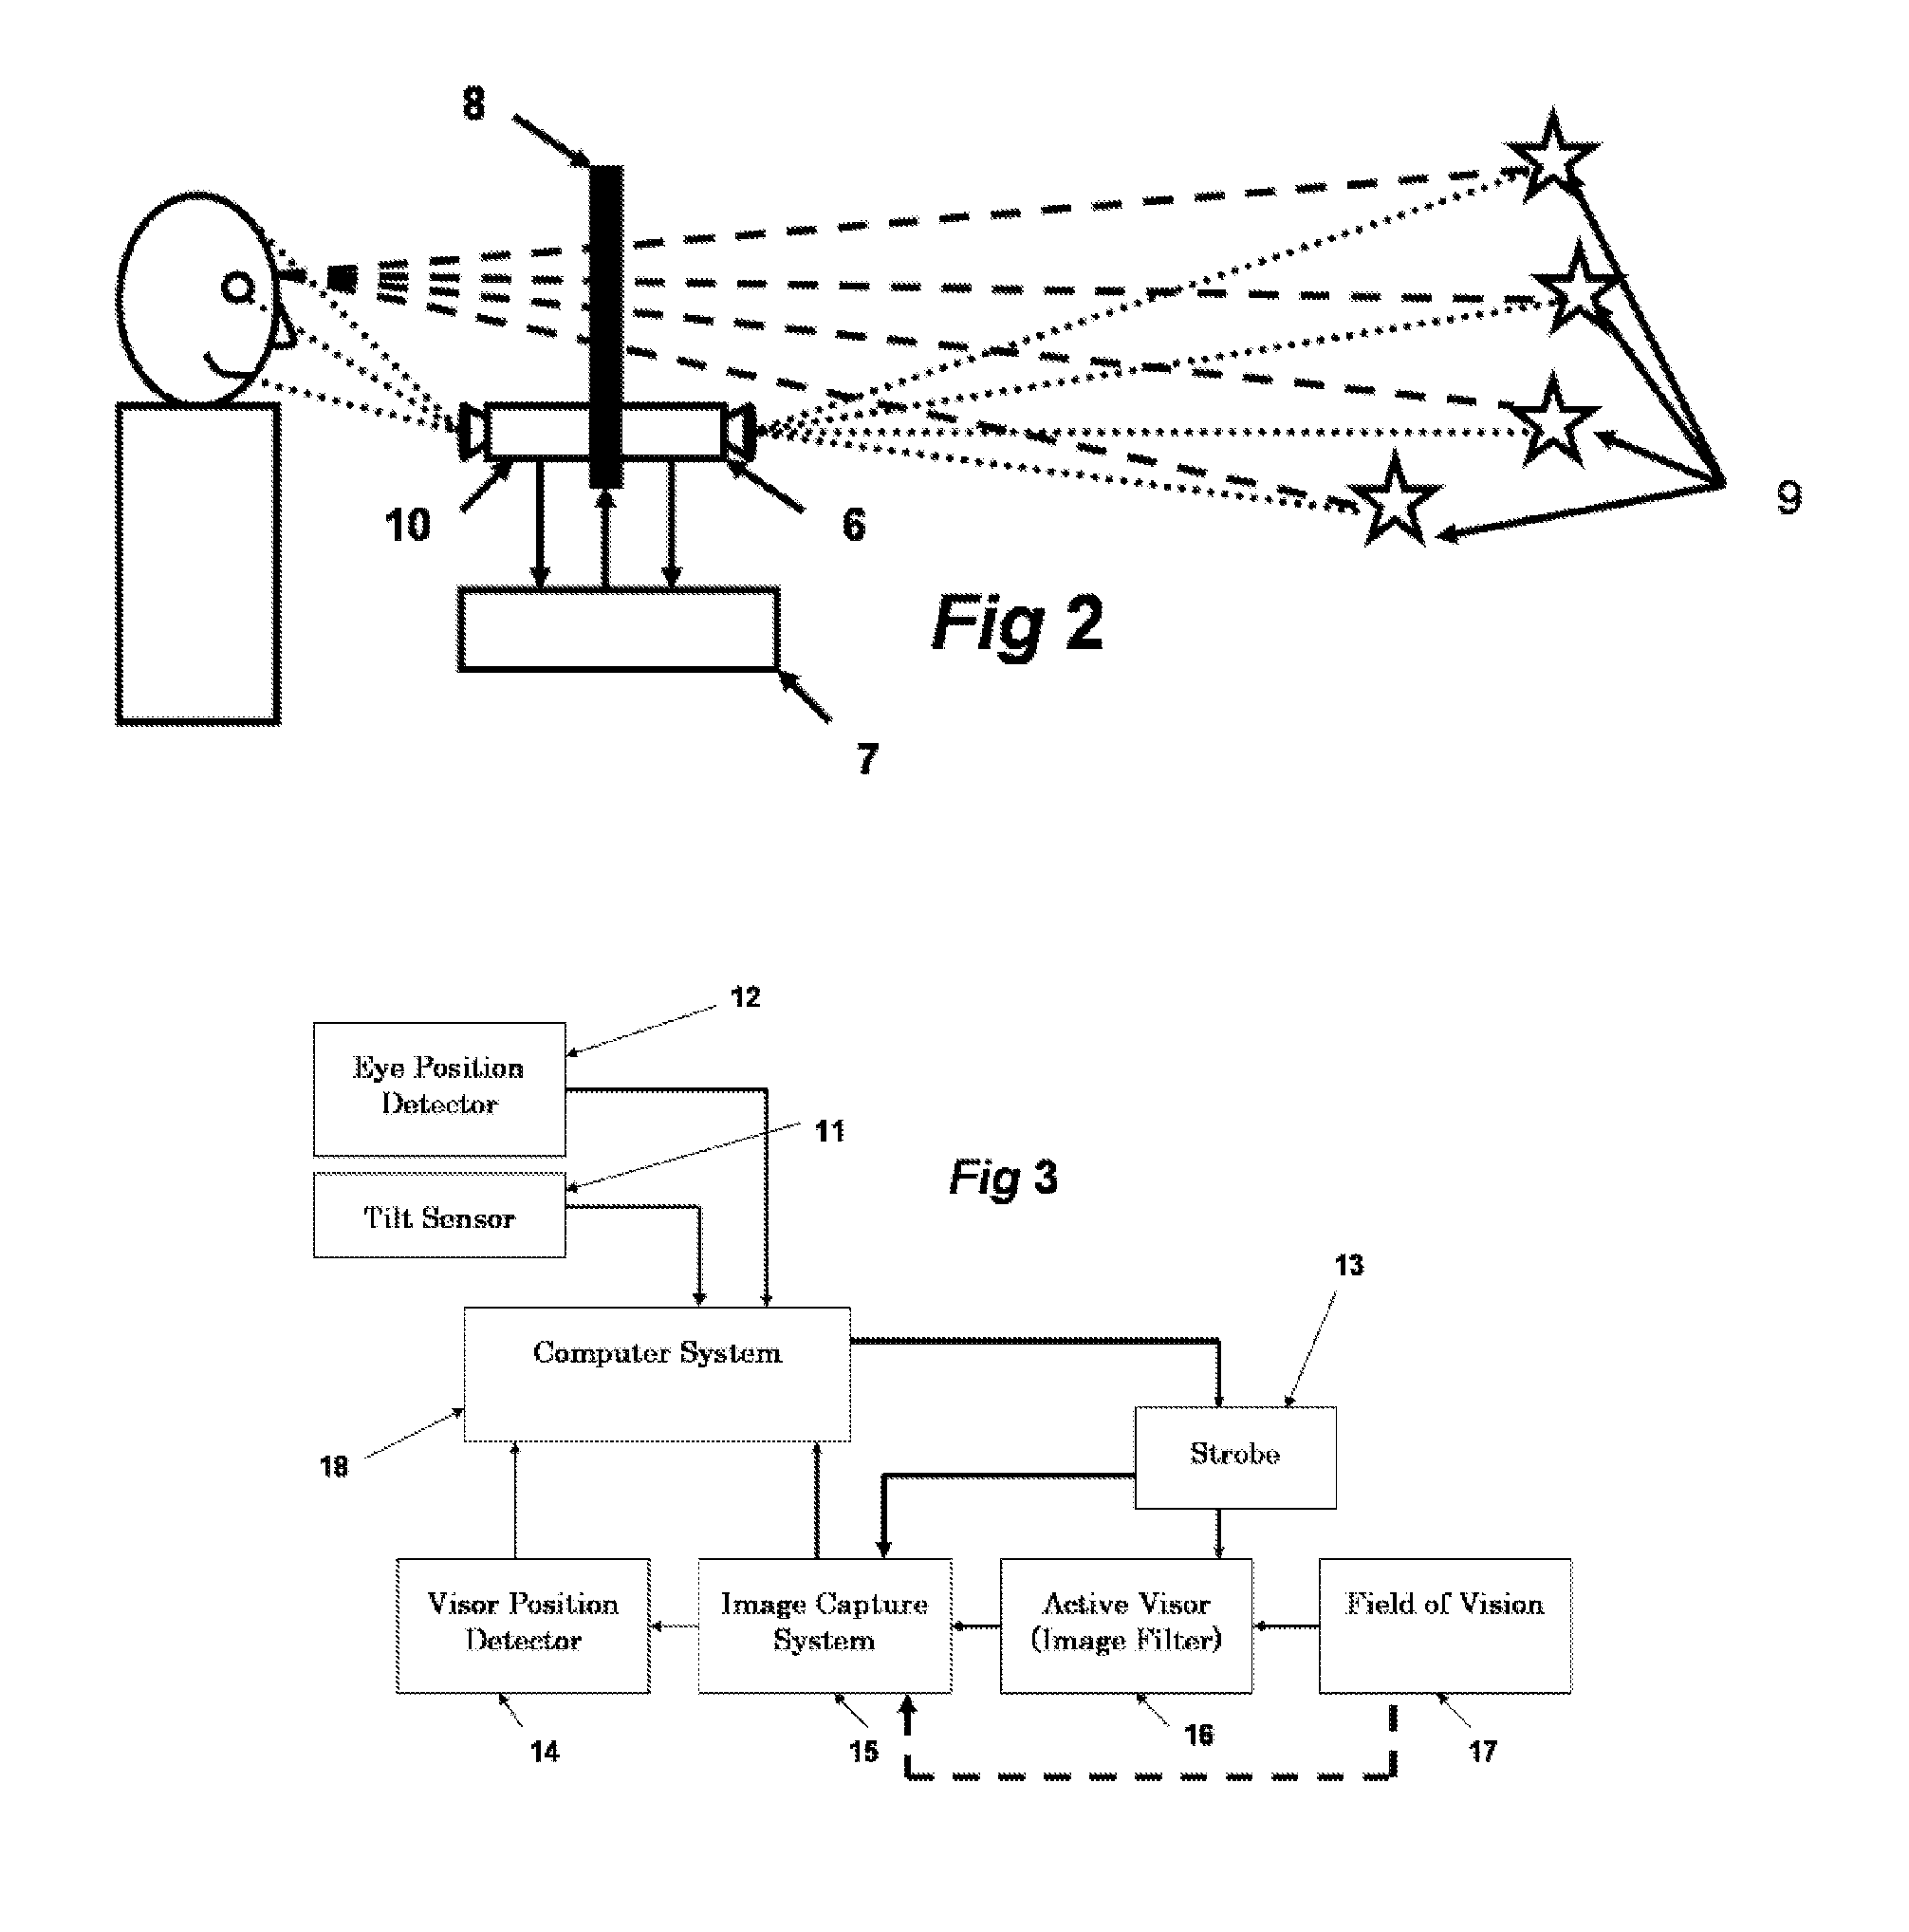
\includegraphics[width=0.7\textwidth]{slike/patent1}
    \captionsetup{font={small}}
    \caption{Prikaz skice izuma iz patenta US2006140502A1 \cite{Allan2006}}
    \label{fig:patent1}
\end{figure}

\flushleft Komponente izuma su:
\justifying
\begin{itemize}[noitemsep]
    \item Aktivna matrica koja će filtrirati svjetlost (broj 8 na slici \ref{fig:patent1}): ovaj izum koristi poseban ekran koji se nalazi ispred vozača. Ovaj ekran može kontrolirati transparentnost svake pojedine točke na površini, slično kao LCD ekran na računalnom monitoru,
    \item Sustav za snimanje slika (broj 6 i 10 na slici \ref{fig:patent1}): u vozilu su postavljeni jedan ili više fotoaparata (kamera) koji snimaju vidno polje vozača. Kamere mogu bilježiti sve što vozač vidi tijekom vožnje,
    \item Detektor položaja zaslona (broj 7 na slici \ref{fig:patent1}): sustav također uključuje senzore koji prate položaj svjetlosnog filtera (ekrana) ispred vozača. Ovi senzori omogućuju sustavu da zna gdje se ekran nalazi u odnosu na vozačeve oči,
    \item Mikrokontroler (broj 18 na slici \ref{fig:patent1}): središnji dio ovog izuma je mikrokontroler, računalna jedinica koja prima informacije iz kamera i senzora. Mikrokontroler obrađuje ove podatke i donosi odluke o tome koje dijelove svjetlosnog filtera treba kontrolirati kako bi smanjio zasljepljujuće svjetlo. \cite{Allan2006}
\end{itemize}

\flushleft Izum radi na sljedeći princip:
\justifying
\begin{itemize}[noitemsep]
    \item Kamere snimaju ono što se nalazi ispred vozača, uključujući i svjetlosne izvore koji uzrokuju zasljepljivanje,
    \item Mikrokontroler analizira sliku koju su kamere snimile i identificira položaj tih svjetlosnih izvora,
    \item Na temelju tog položaja, mikrokontroler aktivira određene dijelove aktivne matrice svjetlosnog filtera. To znači da će ekran postati manje transparentan ili čak potpuno neproziran na mjestima gdje je svjetlosni izvor identificiran,
    \item Vozač tada vidi okolinu kroz ekran, ali svjetla koja bi ga mogla zaslijepiti bit će zamagljena ili blokirana. To omogućuje vozaču da zadrži jasnu vidljivost, čak i ako su mu uperena jak svjetla. \cite{Allan2006}
\end{itemize}

Postoji i patent koji prikazuje jednostavniji izum gdje nisu potrebne kamere, nego vozač ručno klikom na LCD matricu odabire mjesto zatamnjivanja kako bi spriječio zasljepljujuću svjetlost \cite{Broude2009}.

\subsubsection{General Motors Patent US11557234B1: Elektromatsko vjetrobransko staklo i AR}

General Motors je među vodećim kompanijama u autoindustriji \cite{GeneralMotors} koja razvija tehnologiju automatskog zatamnjivanja vjetrobranskog stakla, a koja predstavlja značajan napredak u automobilskoj industriji. Ovaj sustav koristi kameru montiranu na retrovizoru kako bi otkrio kut sunca ili druge svjetlosti i liniju pogleda vozača. Zatim prilagođava nijansu vjetrobranskog stakla kako bi blokirao odsjaj i poboljšao vidljivost. \cite{GeneralMotors2022}

Ova tehnologija koristi elektrokromatski materijal unutar vjetrobranskog stakla koji može promijeniti svoju boju i prozirnost kada se na njega primijeni električni napon. Ovo omogućuje sustavu da brzo i precizno prilagodi nijansu vjetrobranskog stakla kako bi blokirao odsjaj sunca. Osim što poboljšava vidljivost, ova tehnologija također može poboljšati udobnost vožnje. Vozači više ne moraju neprestano podešavati štitnik za sunce ili mijenjati položaj kako bi izbjegli odsjaj sunca. \cite{Bogdan2023}

Ono što čini GM-ovu tehnologiju automatskog zatamnjivanja vjetrobranskog stakla još impresivnijom jest njezina kompatibilnost s proširenom stvarnošću (engl. \emph{augmented reality - AR}) jer će biti moguće upravljanje elektromatskog stakla pomoću napona. Povezivanjem elektrokromnog stakla s AR prikazom na vjetrobranskom staklu, vozačima se nudi poboljšano iskustvo vožnje noću. AR prikaz može pružiti informacije o navigaciji, brzini, upozorenjima i drugim relevantnim podacima izravno na staklu \cite{TudoseSergiu2022}. Ovo znači da vozači ne moraju odvajati pogled s ceste kako bi provjerili svoje instrumente ili navigaciju. Osim što pruža korisne informacije, AR prikaz može dodatno poboljšati sigurnost. Na primjer, sustav može naglasiti prepoznavanje pješaka ili drugih vozila na cesti, pružajući vozačima brže i učinkovitije informacije o potencijalnim opasnostima. \cite{Bogdan2023} \cite{GeneralMotors2022}

Trenutno, General Motors nastavlja razvijati ovu tehnologiju i istražuje mogućnosti za njenu implementaciju u budućim modelima automobila \cite{Bogdan2023}. Cilj je pružiti vozačima sigurniju i ugodniju vožnju, smanjujući utjecaj odsjaja svjetlosti. Kroz inovativnu upotrebu elektrokromatskih materijala i naprednih algoritama za praćenje, ova tehnologija pruža efikasno rješenje za problem odsjaja svjetlosti tijekom vožnje.

Kompanija Apple također pokušava napraviti slično riješenje te je napisala patent \newline US20180304727A1 \cite{OwenMal2018} \cite{Apple2016}. U autoindustriji postoje još i ogledala odnosno retrovizori koji su napravljeni od elektromatskih materijala koji kada su obasjani jakom svjetlošću ne reflektiraju je \cite{Daniel2022}. Još neki od patenata i radova koji su bavili elektromatskim materijalima protiv svjetlosnog zasljepljivanja su: \cite{KumarB2020}, \cite{Dewayne}, \cite{Yuter2010}.

\subsection{Sustavi namjenjeni zaštiti ostalih vozača - ADB sustav}

Samsung PixCell LED svjetlosno rješenje je sustav prilagodljivih dugih svjetala (engl. \emph{Adaptive driving beam systems - ADB systems}) predstavlja naprednu tehnologiju koja se koristi u svjetlosnim sustavima vozila kako bi se poboljšala sigurnost i udobnost vožnje noću. Ta tehnologija koristi mikro LED diode kako bi poboljšala vidljivost i sigurnost na cestama te takav sustav koristi tisuće malih LED dioda (slika \ref{fig:adb}) koje se mogu neovisno kontrolirati kako bi se stvorio precizan snop svjetla što omogućuje automobilima da automatski prilagode intenzitet i smjer svjetlosnih snopova prednjih svjetala kako bi se minimizirao odsjaj i ometanje drugih vozača na cesti, čime se znatno poboljšava sigurnost na cestama. \cite{Samsung2021}

\begin{figure}[h!]
    \centering
    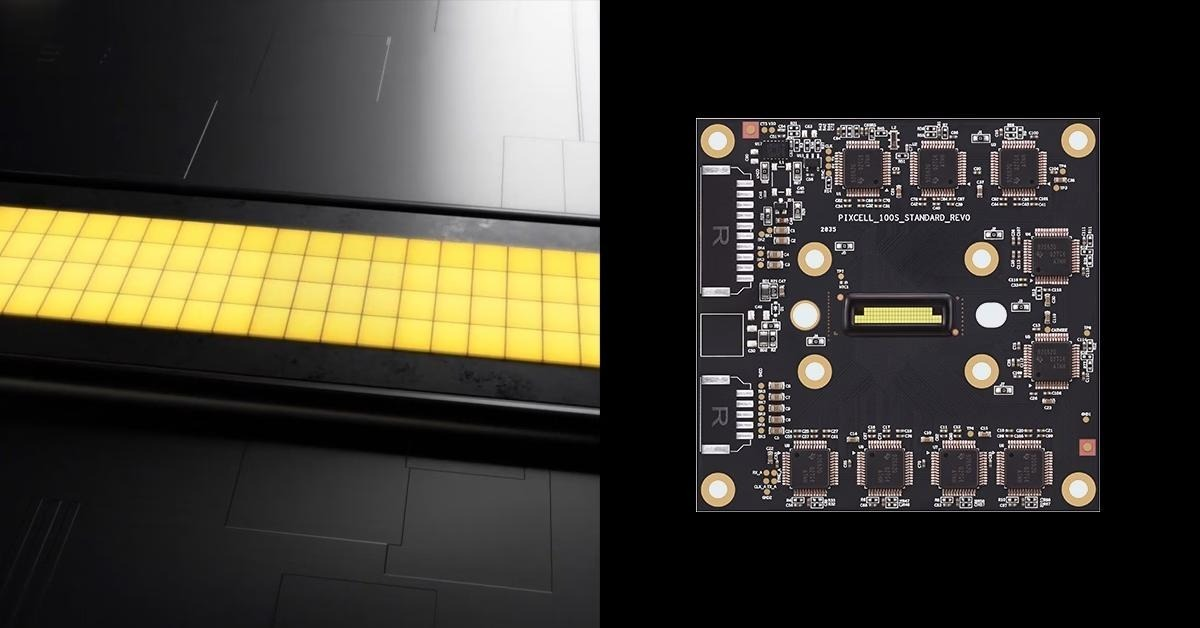
\includegraphics[width=0.7\textwidth]{slike/adb}
    \captionsetup{font={small}}
    \caption{Prikaz pločice sa mikroprocesorima i LED diodama - Samsung PixCell \cite{Samsung2021}}
    \label{fig:adb}
\end{figure}

Jedna od ključnih značajki PixCell LED sustava i općenito ADB sustava je njegova sposobnost prilagodbe snopa svjetla u stvarnom vremenu (Slika \ref{fig:adb2}). Sustav koristi različite senzore, mikrokontrolere, uključujući kamere i senzore osvjetljenja kako bi neprekidno promatrao okoliš i prilagodio snop svjetla kako bi se izbjegao odsjaj za druge vozače. To može poboljšati sigurnost na cestama smanjujući rizik od privremenog sljepila uzrokovanog odsjajem svjetala. \cite{Samsung2021}

\begin{figure}[h!]
    \centering
    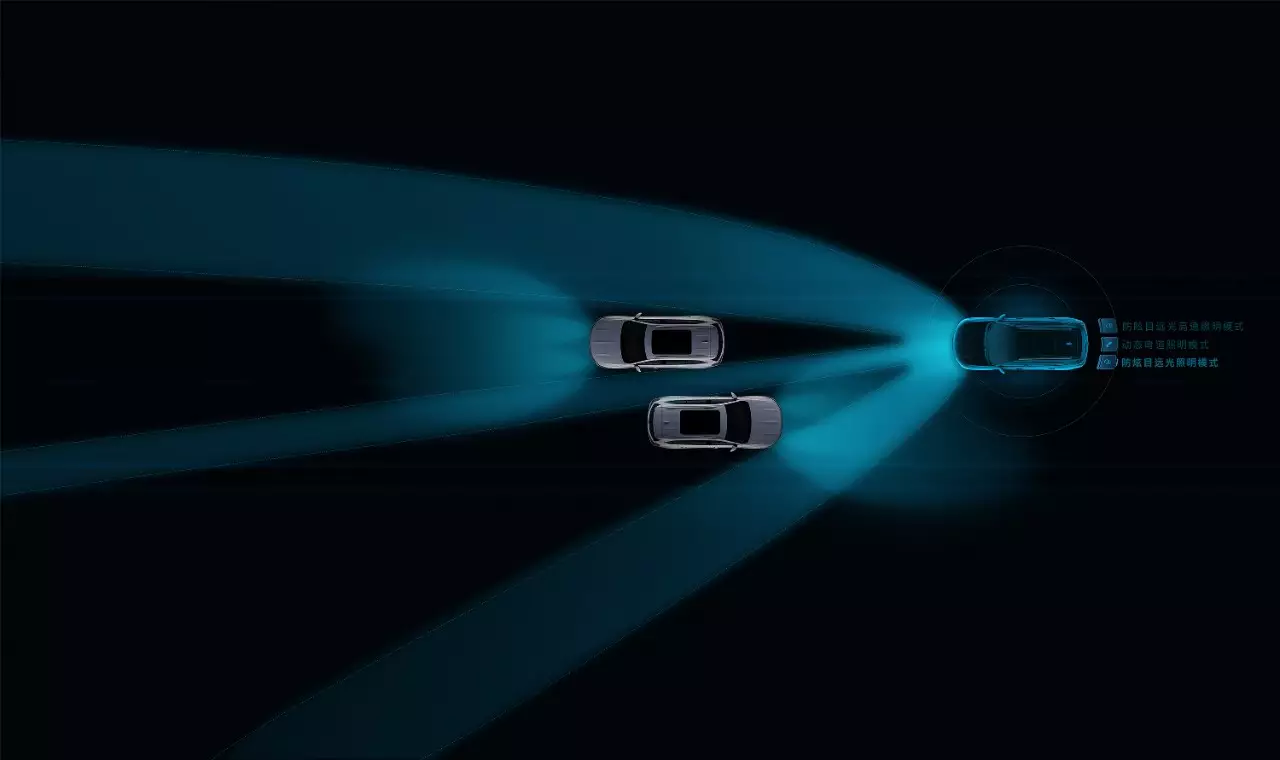
\includegraphics[width=0.7\textwidth]{slike/adb2}
    \captionsetup{font={small}}
    \caption{Prikaz upravljenih svjetlosnih snopova dugih svjetala u cilju zaštite ostalih vozača \cite{Sakalas2021}}
    \label{fig:adb2}
\end{figure}

Jedna od ključnih prednosti ADB sustava je to što vozači ne moraju ručno prebacivati između dugih i kratkih svjetala kako bi izbjegli ometanje drugih vozača. Sustav to radi automatski i trenutačno, što vozačima omogućuje da ostanu fokusirani na cestu bez potrebe za čestim prilagodbama svjetala. Osim toga, ADB sustav također može pružiti dodatnu udobnost vožnje. Primjerice, može prilagoditi svjetlosne snopove tako da osvijetle cestu oko zavoja prije nego što vozač okrene volan, čime se poboljšava preglednost u krivinama \cite{Brahmbhatt2022}, što je prikazano slikom \ref{fig:adb3}.

\begin{figure}[h!]
    \centering
    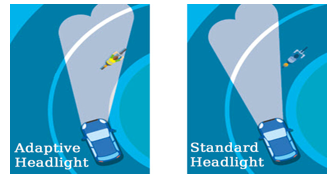
\includegraphics[width=0.5\textwidth]{slike/adb3}
    \captionsetup{font={small}}
    \caption{Razlika u osvjetljenju prilagodljivih i standardnih dugih svjetala \cite{Brahmbhatt2022}}
    \label{fig:adb3}
\end{figure}

Važno je napomenuti da je ADB tehnologija postala sveprisutna u novijim automobilima, posebno u onima visoke klase. To je jedan od primjera kako tehnološki napredak u automobilskoj industriji kontinuirano doprinosi sigurnosti i udobnosti vožnje, posebno u uvjetima smanjene vidljivosti kao što su noćna vožnja ili loše vremenske prilike. Popularne kompanije u autoindustriji Ford i Audi također razvijaju sličnu ADB tehnologiju. \cite{ElectronicSpecifier2016}

\chapter{Izrada sustava}

U ovom poglavlju će biti opisana izrada i testiranje prilagodljivog sustava za smanjenje svjetlosnog zasljepljivanja vozača. Slika \ref{fig:arhit_hard_soft} prikazuju hardversku (brojevi 1, 2, 3 i 4) i softversku (brojevi 5 i 6) arhitekturu prototipa. Opis izrade će biti podijeljen na četiri potpoglavlja od kojih će svaki opisivati određenu komponentu budući da se sustav sastoji od četiri komponente:
\begin{itemize}[noitemsep]
    \item procesna jedinica (laptop) i hardver (web kamere i LCD matrica),
    \item komponenta za prepoznavanje i pozicioniranje izvora svjetla,
    \item komponenta za prepoznavanje i pozicioniranje očiju vozača,
    \item komponenta za polarizaciju LCD matrice kao reaktivne komponente.
\end{itemize}

\begin{figure}[h!]
    \centering
    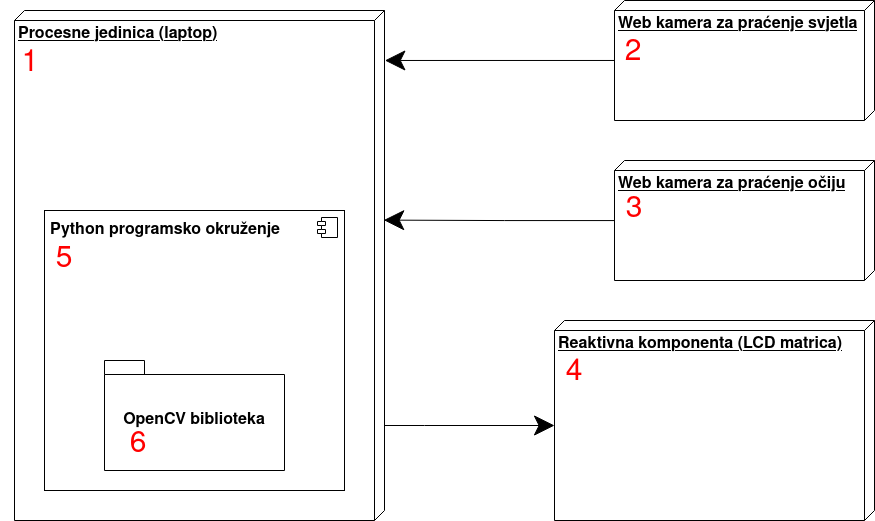
\includegraphics[width=0.8\textwidth]{slike/arhit_hard_soft}
    \captionsetup{font={small}}
    \caption{Hardverska i softverska arhitektura prototipa [autorski rad]}
    \label{fig:arhit_hard_soft}
\end{figure}


Programski kod koji se bude prikazivao u radu može se pronaći na GitHub repozitoriju preko poveznice: \url{https://github.com/StjepanPetrovic/Prilagodljiv-sustav-za-smanjenje-svjetlosnog-zasljepljivanja-vozaca}. Svi isječci programskog koda su uzeti iz jedne datoteke \href{https://github.com/StjepanPetrovic/Prilagodljiv-sustav-za-smanjenje-svjetlosnog-zasljepljivanja-vozaca/blob/main/development/main.py}{$main.py$} te će se u isječcima programskog koda moći vidjeti i redni brojevi linija koda koji se odnose na redne brojeve linija koda iz datoteke \href{https://github.com/StjepanPetrovic/Prilagodljiv-sustav-za-smanjenje-svjetlosnog-zasljepljivanja-vozaca/blob/main/development/main.py}{$main.py$}.

Ovim radom izrađen je prototip koji će objasniti i prikazati ideju za izradu ovakvog sustava, ali ovaj prototip nije spreman za upotrebu u stvarnoj okolini. Ono što nije ovim radom obrađeno je navedeno u nastavku, to su neke od glavnih značajki koje bi sustav trebao ispunjavati kako bi pronašao svrhu u stvarnoj okolini:
\begin{itemize}[noitemsep]
    \item korištenje mikroprocesora koji će biti zadužen samo za obavljanje funkcionalnosti sustava,
    \item korištenje posebno izrađene prozirne LCD matrice ili korištenje drugog medija kao reaktivne komponente koja bi poslužila svrsi,
    \item korištenje posebnog modela i senzora za otkrivanje jačine svjetlosti,
    \item korištenje posebno istreniranog modela ili senzora koji će moći izračunati udaljenost zasljepljujućeg svjetla i očiju od reaktivne komponente,
    \item korištenje algoritma koji će uzeti u obzir sve udaljenosti, nagib vjetrobranskog stakla i klasifikacije objekata od interesa kako bi što kvalitetnije izračunavao mjesto na kojemu treba zaustaviti svjetlost preko reaktivne komponente,
    \item spremnost na rad u noćnim uvjetima,
    \item velika količina testiranja sustava u raznovrsnoj i dinamičnoj okolini (posebno noćnoj okolini).
\end{itemize}

\section{Komponenta procesne jedinice i hardver}

Ovo poglavlje opisuje komponentu procesne jedinice kao komponentu koja čini temelj i softverski povezuje ostale komponente, a također opisuje i kako je sustav hardverski povezan.

\subsection{Hardver}
U ovom radu komponentu procesne jedinice predstavlja laptop (broj 1 na Slici \ref{fig:arhit_hard_soft}) na kojem će se izvršavati programski kod i čiji će procesor obrađivati ulazne informacije koje šalju kamere (broj 2 i 3 na Slici \ref{fig:arhit_hard_soft}), a kamere su obične web kamere od kojih je jedna ugrađena u laptop, a druga je eksterna i priključena je preko USB priključka u laptop. Jedna kamera je namjenjena za snimanje okoline ispred vozača, a druga kamera je namijenjena za snimanje samog vozača.

Ispred vozača bi se nalazila LCD matrica (broj 4 na Slici \ref{fig:arhit_hard_soft}) koja će smanjiti i sprječiti zasljepljujuću svjetlost da dođe do očiju vozača. LCD matrica, zajedno sa elektronikom, za ovaj rad je izvađena iz običnog monitora te povezana preko HDMI priključka u laptop i ponaša se kao drugi prošireni zaslon laptopa. Na slici \ref{fig:lcd_matrica_1} i \ref{fig:lcd_matrica_2} može se vidjeti kako izgleda LCD matrica zajedno sa elektronikom i priključcima kada je izvađena iz monitora i postavljena u postolje kako bi uspravno stojala prilikom testiranja prototipa.

\begin{figure}[h!]
    \centering
    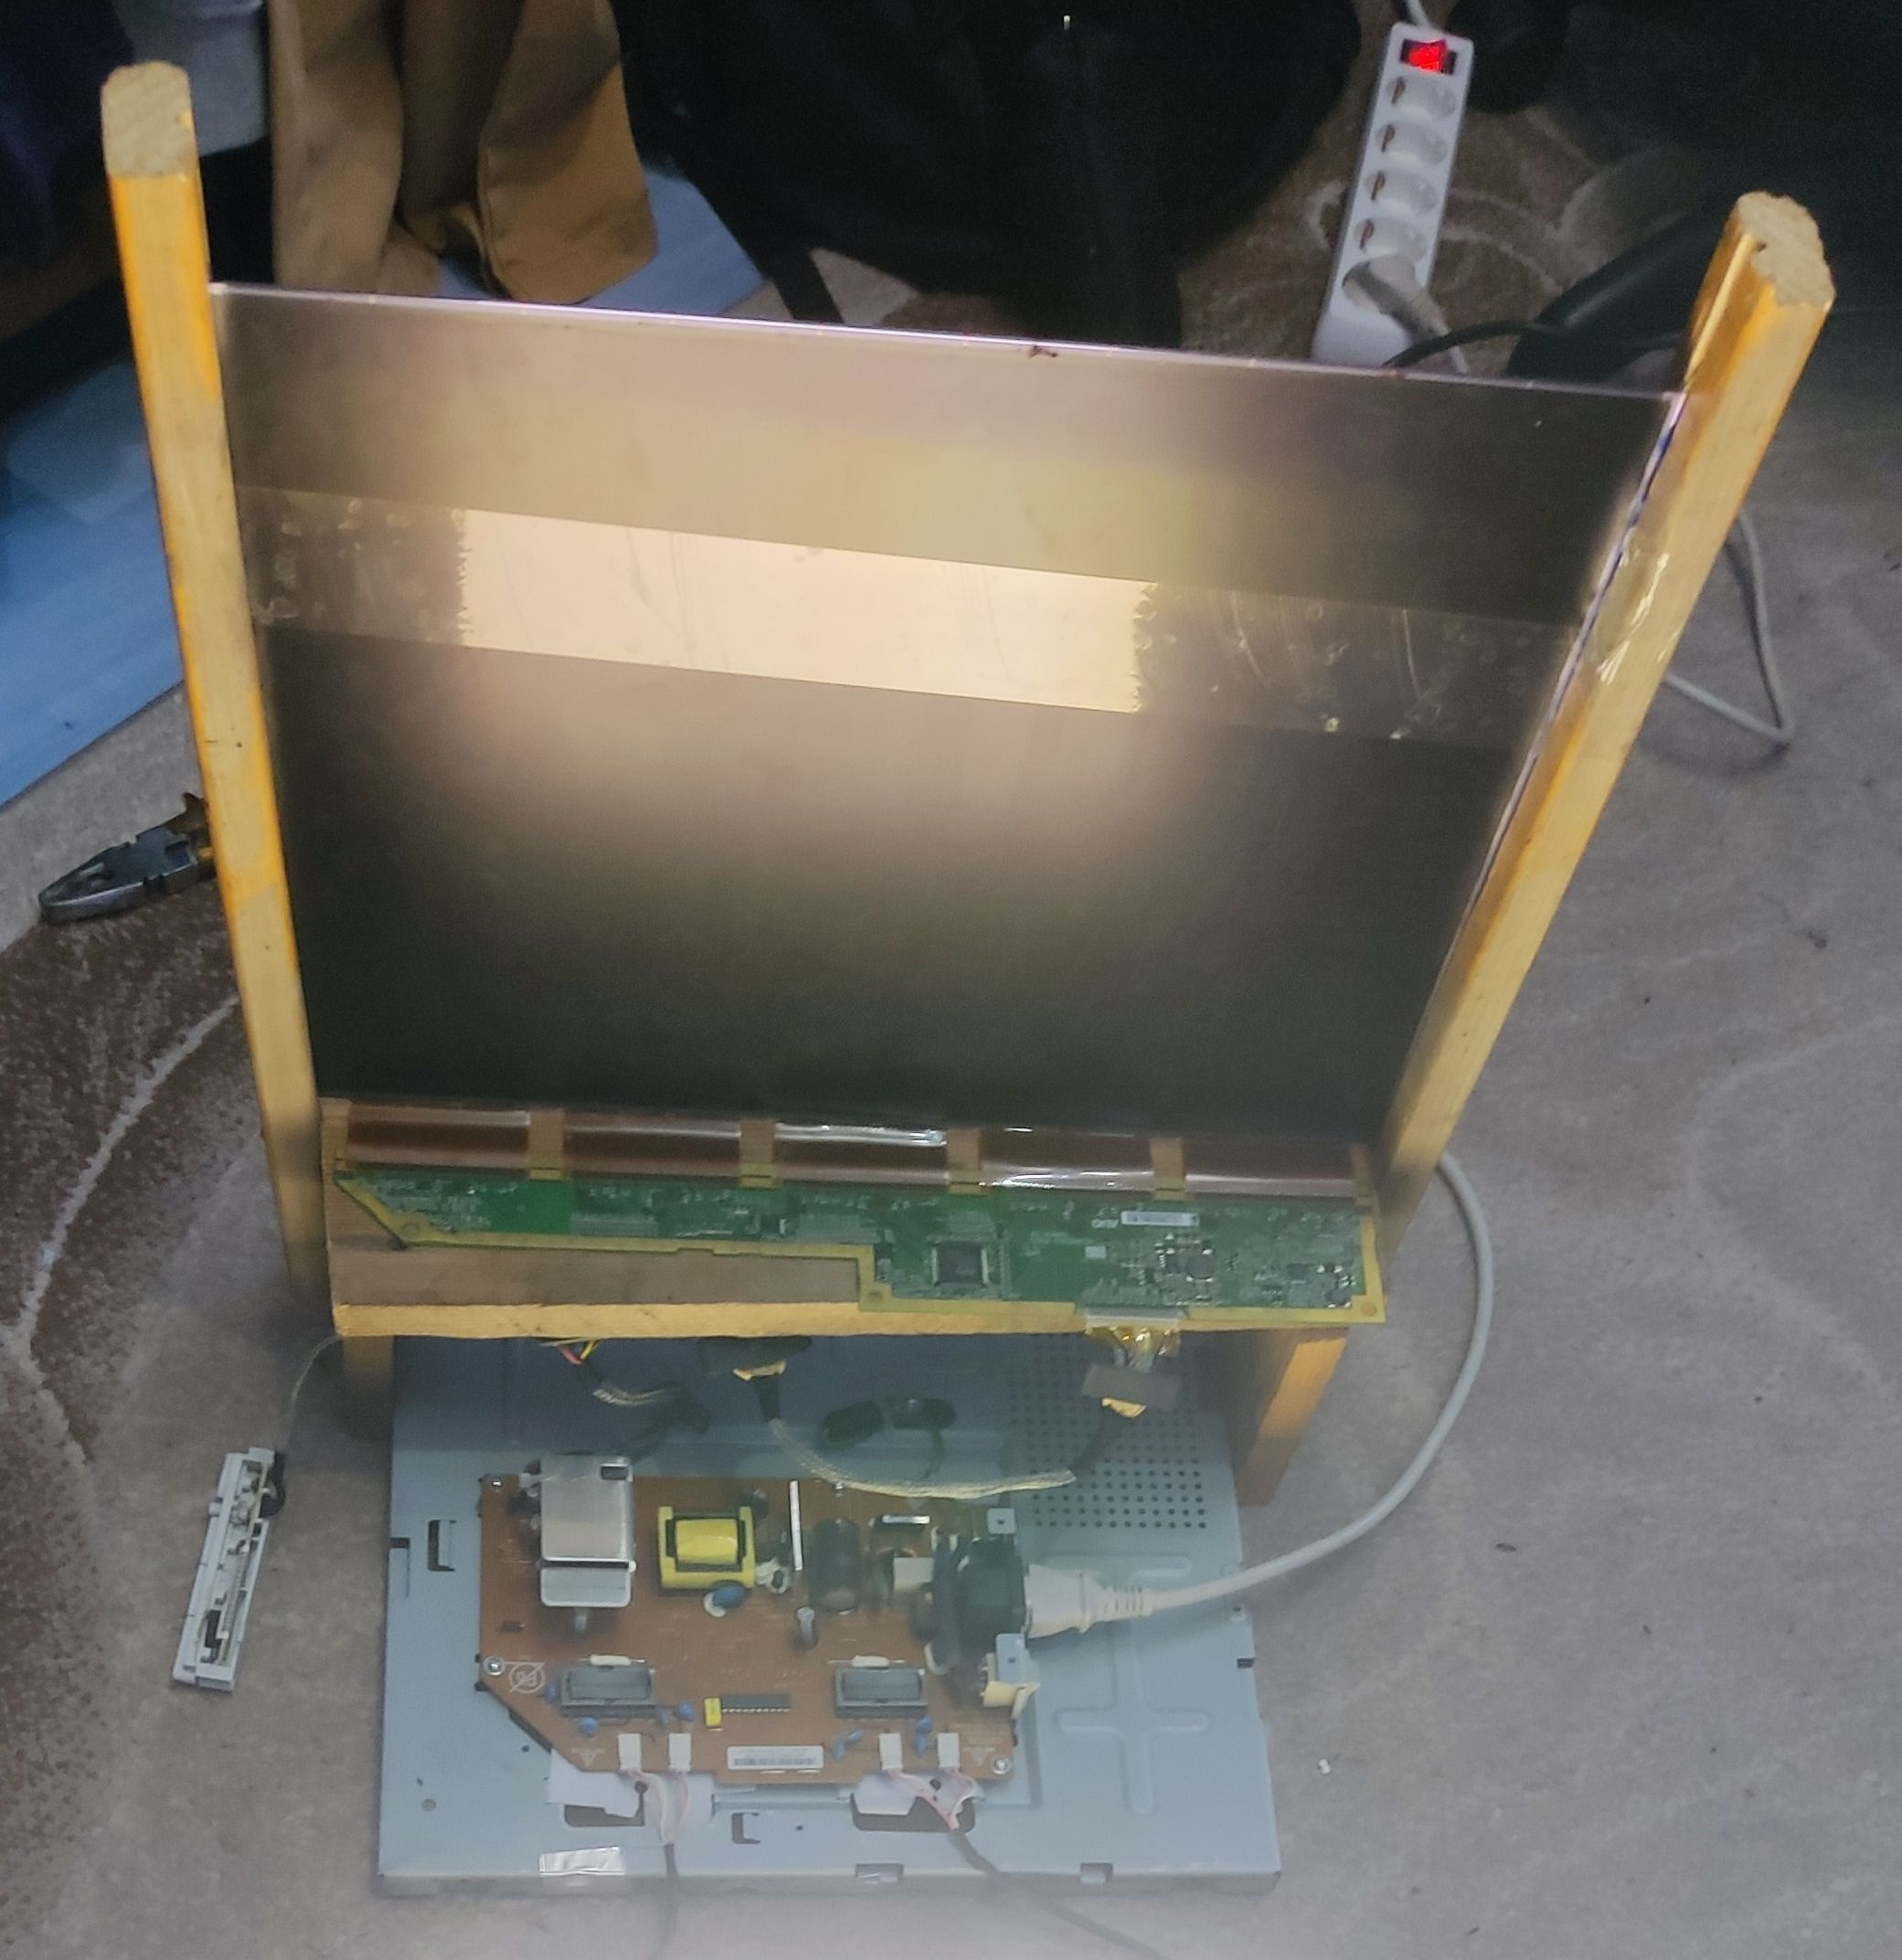
\includegraphics[width=0.4\textwidth]{slike/lcd_matrica_1}
    \captionsetup{font={small}}
    \caption{Prikaz LCD matrica s prednje strane kada je izvađena iz monitora [autorski rad]}
    \label{fig:lcd_matrica_1}
\end{figure}

\begin{figure}[h!]
    \centering
    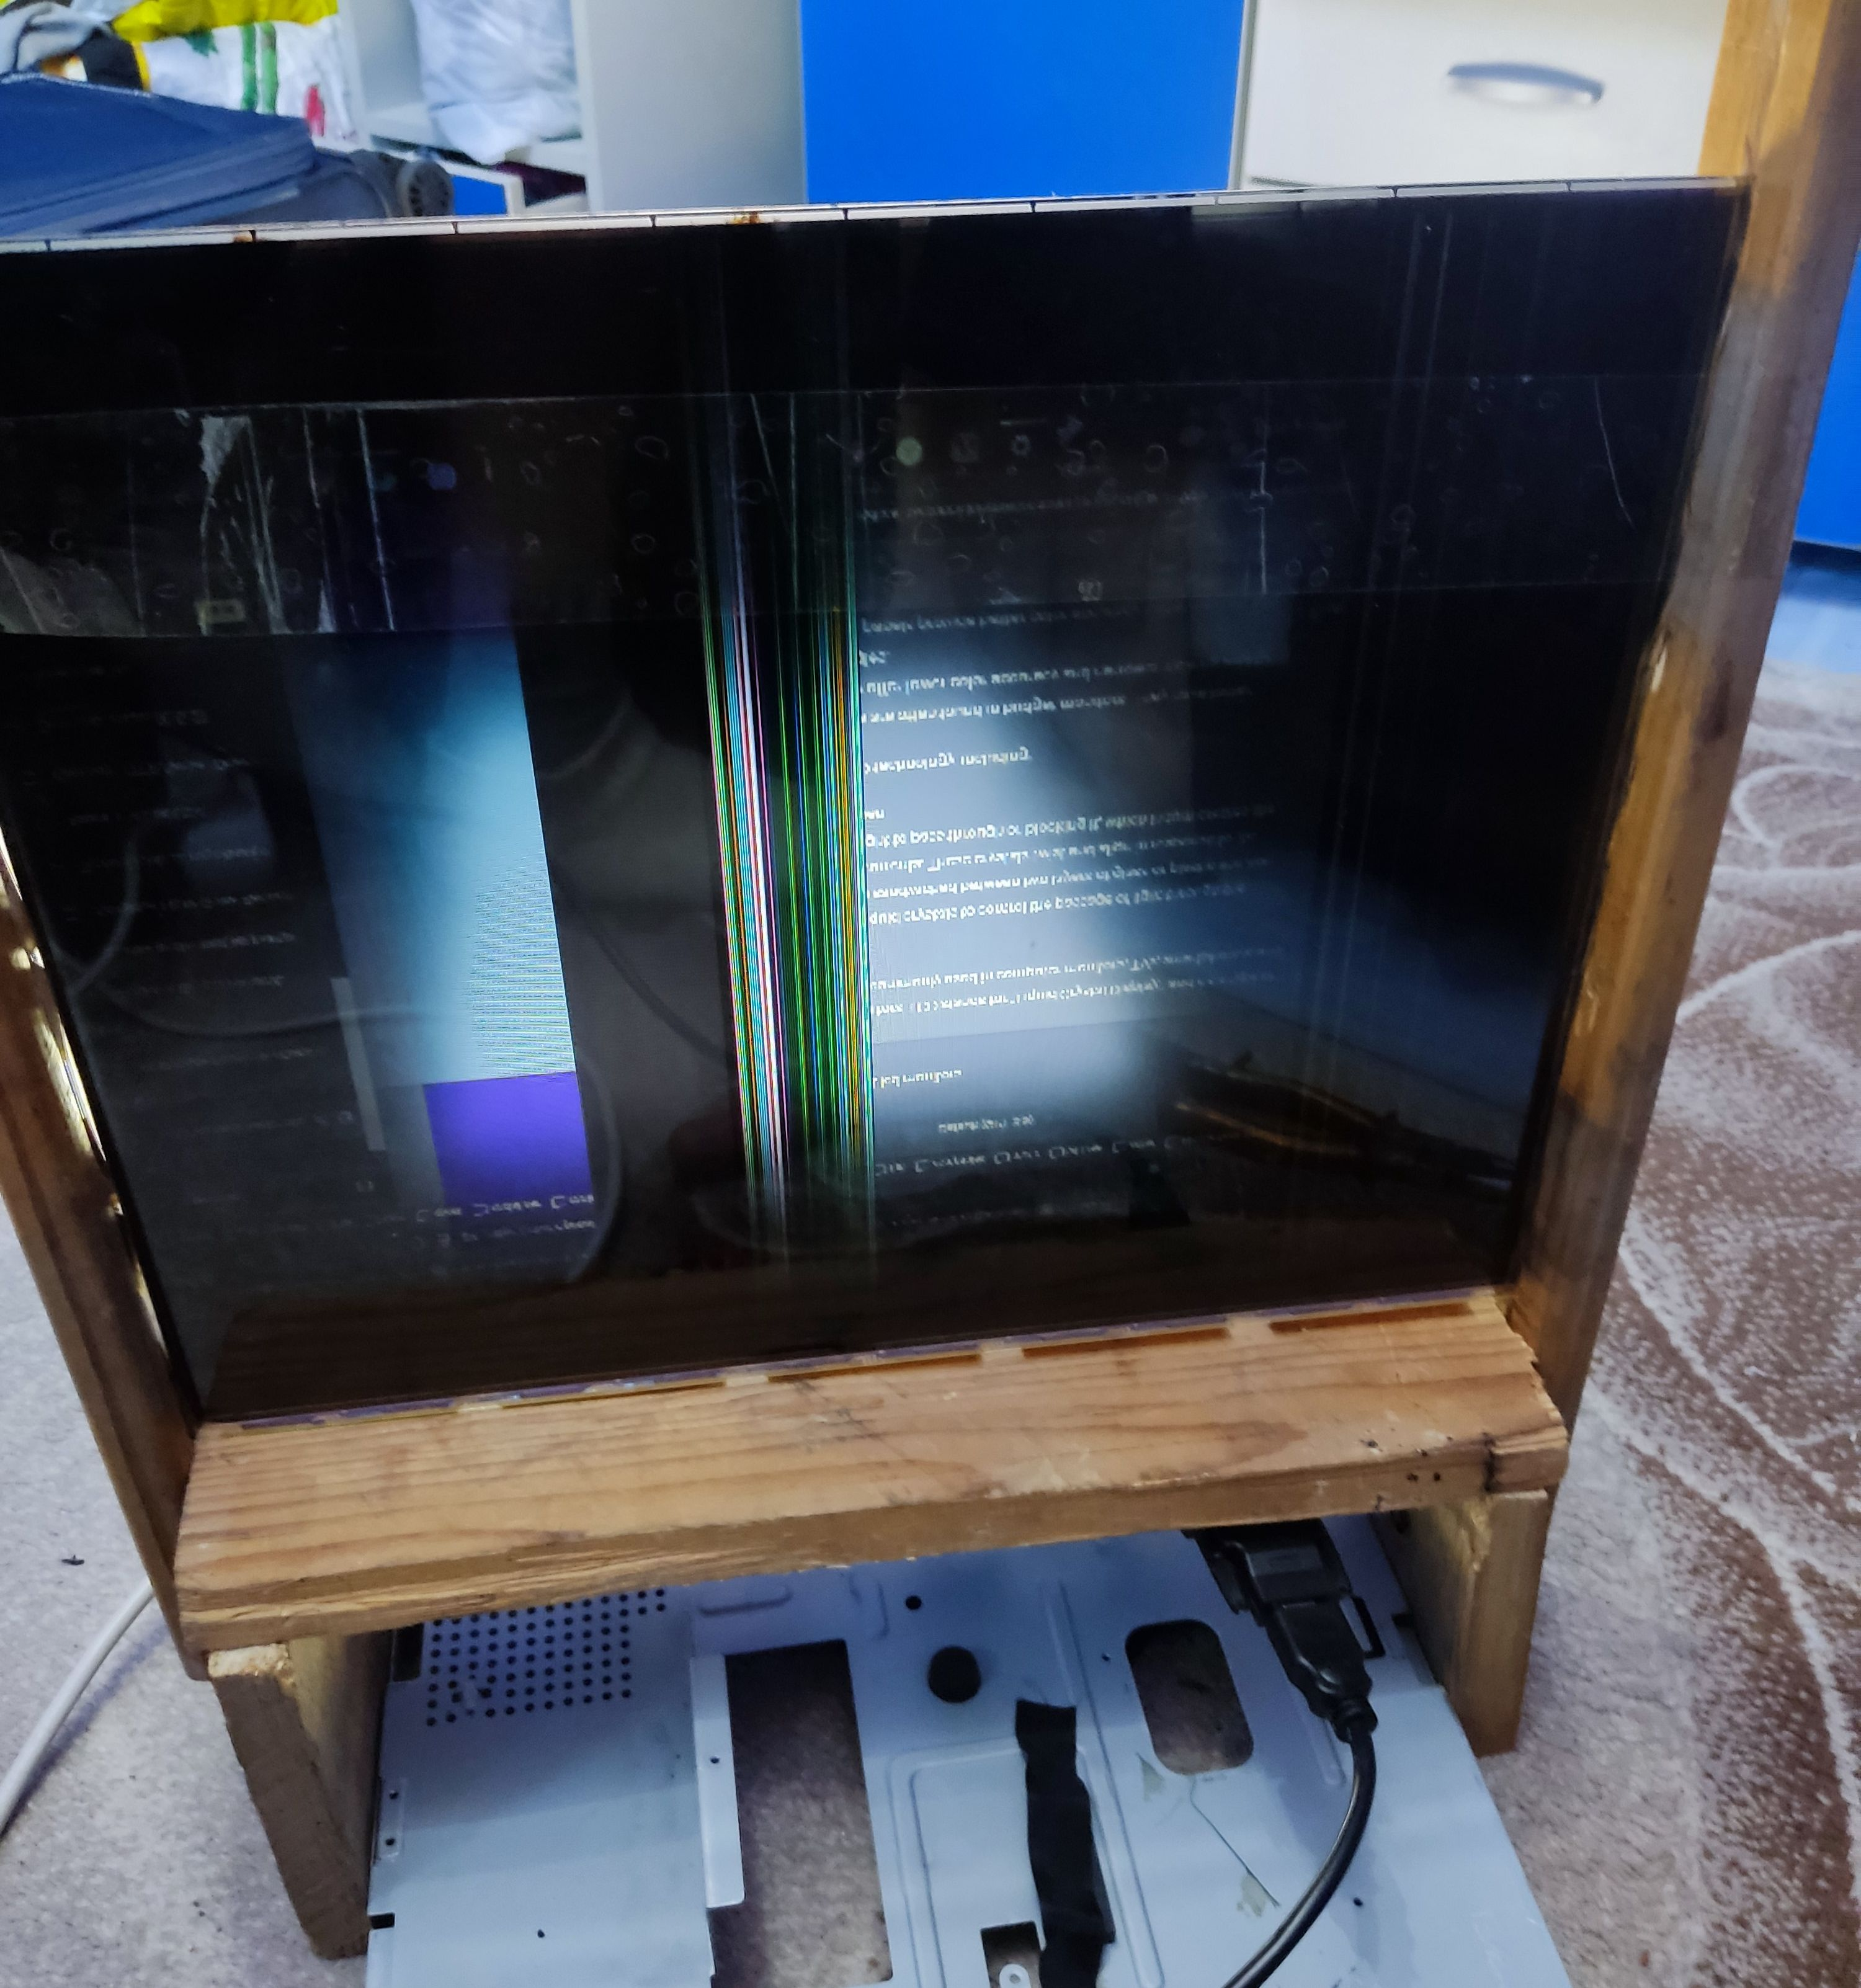
\includegraphics[width=0.4\textwidth]{slike/lcd_matrica_2}
    \captionsetup{font={small}}
    \caption{Prikaz LCD matrica sa zadnje strane kada je izvađena iz monitora [autorski rad]}
    \label{fig:lcd_matrica_2}
\end{figure}

\newpage
\subsection{OpenCV-Python biblioteka}

Budući da je potrebno prepoznati i pronaći točne pozicije na kojima se nalaze objekti od interesa odnosno svjetlost i oči, potrebno je koristiti algoritme za računalni vid. Kako IBM navodi (engl. \emph{International Business Machines Corporation - IBM}), računalni vid je grana umjetne inteligencija (engl. \emph{Artificial intelligence - AI}) koja omogućava računalima da pruže smislene informacije koje pronađu obradom slika, videa ili drugog vizualnog izvora te da reagiraju shodno toj informaciji \cite{cv-ibm}. Stoga kako bi mogli pronaći pozicije svjetlosti i očiju na okvirima koji se budu dobivali od kamera, u ovom radu koristit će se biblioteka OpenCV za programski jezik Python.

OpenCV je biblioteka otvorenog koda (engl. \emph{open source}) koja služi za rješavanja problema vezanih za računalni vid (engl. \emph{computer vision}) i strojno učenje (engl. \emph{machine learning}) te pruža često potrebnu infrastrukturu za aplikacije koje integriraju računalni vid \cite{opencv}. OpenCV biblioteka podržava programske jezike C++, Python, Java, itd., i dostupna je na Windows, Linux, OS X, Andorid, iOS platformama. U radu će se koristiti OpenCV-Python biblioteka koja je Python API (engl. \emph{Application Programming Interface - API}) za OpenCV biblioteku koja uzima najbolje kvalitete OpenCV C++ API-ja i Python programskog jezika \cite{opencv-python}.

Treba se uzeti u obzir da je Python sporiji programski jezik u odnosu na C++ koji je se također mogao koristiti u ovom radu, no moguće je imati i Python module koji će sadržavati C++ programski kod za procesorski intenzivne zadatke, a rezultat toga je da se izvršavanja Python programskog koda izvršava približno jednakom brzinom kao i brzina izvršavanja C++ programskog koda jer se C++ kod izvršava u pozadini te lakše je programirati u Python programskom jeziku nego u C++ programskom jeziku \cite{opencv-python}.

Kako bi se koristila biblioteka OpenCV sa programskim jezikom Python potrebno ju je prvo instalirati. U terminalu unesite komandu: $pip$ $install$ $opencv$-$python$ i OpenCV biblioteka će biti instalirana. Ako ju želite korisiti u $conda$ radnom okruženju koje nudi dodatne pogodnosti slijediti upute za odgovarajući operativni sustav (engl. \emph{Operating System - OS}) za:
\newpage
\begin{itemize}[noitemsep]
    \item Linux OS: \url{https://youtu.be/gt0Mpi6FFzQ?si=QCLjiDrJcBCP5qV8},
    \item Windows OS: \url{https://youtu.be/RfFiTozvOdQ?si=6jtyHU4YK9jsi6kv},
    \item MacOS: \url{https://youtu.be/hZWgEPOVnuM?si=kD9CNUf4kNqyWBBK},
\end{itemize}
te je potrebno postaviti $conda$ radno okruženje: \url{https://www.jetbrains.com/help/pycharm/conda-support-creating-conda-virtual-environment.html}.

\flushleft Nakon instalacije moguće je uključiti biblioteku pomoću sljedećeg programskog koda \ref{lst:lstlisting_1}:
\justifying
\begin{lstlisting}[language=Python, label={lst:lstlisting_1}, firstnumber=1, style=colored, caption=Uključivanje biblioteke $OpenCV$]
import cv2 as cv
\end{lstlisting}

\justifying

\subsection{Redovi kao struktura podataka za spremanje okvira}

Ono što algoritam za računalni vid uzima kao ulazni podatak je fotografija odnosno okvir (engl. \emph{frame}) koji se dobiva od kamere koja cijelo vrijeme snima okolinu. Slika \ref{fig:slika_frame} objašnjava kako je skup okvira odnosno fotografija fotografiranih uzastopno u kratkom vremenskom periodu jednak videu te na taj način video i nastaje \cite{AnimoticaBlog2020}.

\begin{figure}[h!]
    \centering
    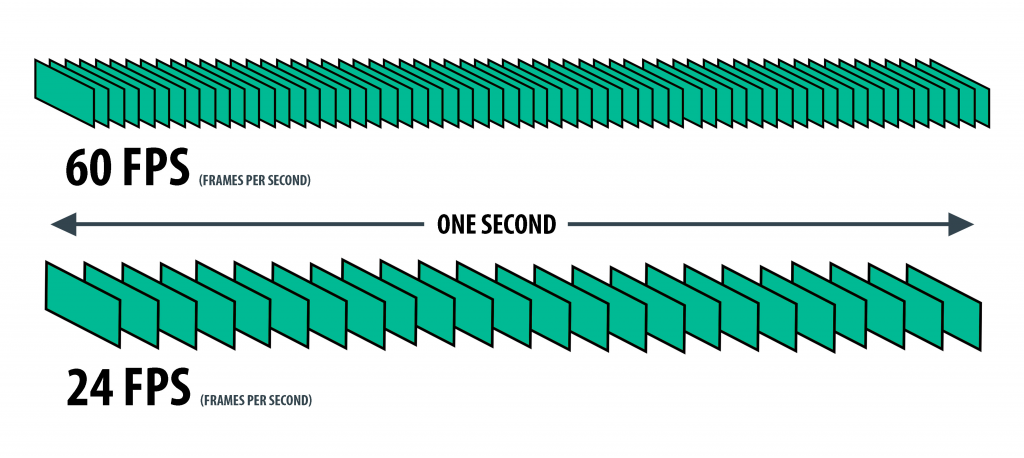
\includegraphics[width=1\textwidth]{slike/frames-per-second-diagram}
    \captionsetup{font={small}}
    \caption{Prikaz uzastopnih fotografija/okvira koji čine video od jedne sekunde \cite{AnimoticaBlog2020}}
    \label{fig:slika_frame}
\end{figure}

Budući da kamere cijelo vrijeme snimaju okolinu, one generiraju mnogo fotografiju u stvarnom vremenu od kojih će program uzimati po jednu fotografiju u određenom trenutku, analizirati ih i spremati ih u posebne strukture podataka za daljnju obradu. U ovom radu strukture podataka koje su uzete za ovu svrhu spremanja potrebnih informacija su redovi (engl. \emph{Queues}) tipa FIFO - "prvi ušao, prvi izašao" (engl. \emph{First In First Out - FIFO}).

Razlog zbog čega su odabrani redovi kao struktura podataka u koju će se spremati podaci je taj što redovi osiguravaju sigurno korištenje podataka između više dretava, a tip FIFO zbog toga što je bitno da se prvo analizira okvir koji je najprije došao \cite{PythonSoftwareFoundation}. To će biti vrlo korisno budući da će ovaj program koristiti glavnu dretvu za čitanje okvira iz redova i njihovo prikazivanje, i drugu dretvu za dobijanje okvira pomoću kamere, analiziranje i njihovo spremanje u redove. Slika \ref{fig:dijagram_red} slikovito prikaziva red kao strukturu podataka te prikaziva funkcije $get()$ i $put()$ klase $Queue$ pomoću kojih se podaci dodavaju i uzimaju iz redova. Programski kod \ref{lst:lstlisting_2} prikazuje kako uključiti biblioteku i inicijalizirati redove.

\begin{figure}[h!]
    \centering
    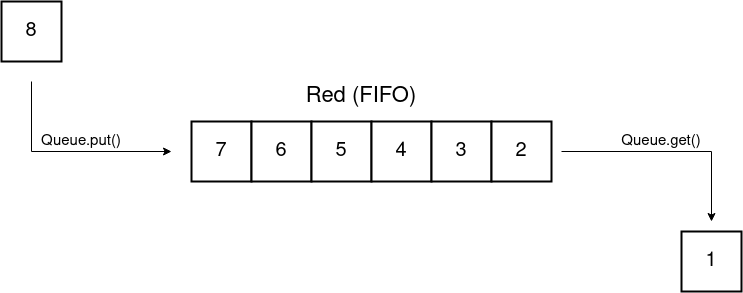
\includegraphics[width=0.7\textwidth]{slike/redovi_dijagram}
    \captionsetup{font={small}}
    \caption{Slikovit prikaz reda kao strukture podataka [autorski rad]}
    \label{fig:dijagram_red}
\end{figure}

\begin{lstlisting}[language=Python, label={lst:lstlisting_2}, firstnumber=4, style=colored, caption=Uključivanje biblioteke $queue$ i inicijaliziranje redova]
from queue import Queue

eyes_frames_queue = Queue()
light_frames_queue = Queue()

eyes_position_queue = Queue()
light_position_queue = Queue()
\end{lstlisting}

Programskim kodom \ref{lst:lstlisting_2} inicijalizirani su  $eyes\_frames\_queue$ i $light\_frames\_queue$ redovi koji služe za spremanje okvira koji se dobiju pomoću kamera i prikazivanje istih okvira nakon njihova analiziranja te još su inicijalizirani $eyes\_position\_queue$ i $light\_position\_queue$ redovi koji služe za spremanje koordinata za pozicije očiju i izvora svjetla koji se dobiju nakon analiziranja okvira i služe za kasnije računanje prilikom stvaranje sloja zaštite koji će se prikazivati na LCD matrici.

Okviri se prikazuju u posebno otvorenim prozorima na zaslonu laptopa i LCD matrice koje otvaramo sa programskim kodom \ref{lst:lstlisting_3}. Prvi prozor prikaziva okvire od kamere koja snima oči vozača, drugi prozor prikaziva okvire od kamere koja snima vanjsku okolinu koja dolazi ususret vozaču, a treći prozor je prozor koji će biti postavljen na LCD matricu i prikazivat će zaštitni okvir koji je ustvari okvir popunjen bijelom bojom, a crnom bojom na mjestima koja su izračunata kako bi se zatamnio određen dio matrice i spriječilo prodiranje svjetlosti. Kontinuirano prikazivanje okvira rezultira time da se može u realnom vremenu pratiti ono što kamere gledaju u obliku videa uživo (engl. \emph{live stream}).

\newpage
\begin{lstlisting}[language=Python, label={lst:lstlisting_3}, firstnumber=142, style=colored, caption=Otvaranje prozora na zaslonu]
def open_window(name):
    cv.namedWindow(name, cv.WINDOW_NORMAL)
    cv.setWindowProperty(name, cv.WND_PROP_AUTOSIZE, cv.WINDOW_NORMAL)


if __name__ == '__main__':
win_name_eyes = 'Eyes Camera Preview'
open_window(win_name_eyes)

win_name_light = 'Light Camera Preview'
open_window(win_name_light)

win_name_protection = 'Protection Preview'
open_window(win_name_protection)
\end{lstlisting}

\subsection{Višedretvenost zbog raspodijele I/O zadataka}

\flushleft Zadatci koje program treba odrađivati su:
\begin{enumerate}[noitemsep]
    \item dohvačanje/čitanje okvira iz video izvora - ulaznog uređaja (kamere),
    \item analiziranje okvira (otkrivanje svjetlosti i očiju),
    \item spremanje pozicija i okvira u redove,
    \item čitanje okvira iz redova,
    \item izračunavanje pozicije koju treba zatamniti na LCD matrici,
    \item prikazivanje okvira u prozorima na zaslonu.
\end{enumerate}

\justifying

Navedeni zadatci su većinom vezani za ulazno/izlazne operacije (engl. \emph{input/output bound - I/O bound}) te ih je sve potrebno izvršavati istovremeno, zbog čega je korisno koristiti dretve kako bi se zadatci podijelili po dretvama koje možemo zamisliti kao dodatne radnike u firmi zbog kojih će se moći obaviti više posla paralelno s ostalim poslom. Dretve donose pojednostavljen dizajn koda i njihovo pravilno implementiranje ne može stvoriti situaciju da jedan zadatak zaustavlja izvođenje ostalih zadataka \cite{AndersonJim}.

U CPython implementaciji treba uzeti u obzir da se zbog GIL-a (engl. \emph{Global Interpreter Lock - GIL}) samo jedna dretva može izvršavati Python programski kod odjednom, a ovo se ograničenje može izbjeći korištenjem specijaliziranih biblioteka, no dojam paralelnosti se ipak postiže visokofrekventnom izmjenom rada nad dretvama. Dretve su prikladne za korištenje kod ulazno/izlaznih operacija, dok se kod procesorski složenijih zadataka savjetuje korištenje procesa \cite{PythonSoftwareFoundation2}. U ovom radu zadatci za analiziranje i izračunavanje nisu procesorski zahtjevni, stoga će ih dretve izvršavati.

\flushleft Potrebno je uključiti biblioteku pomoću sljedećeg programskog koda \ref{lst:lstlisting_thread}:
\begin{lstlisting}[language=Python, label={lst:lstlisting_thread}, firstnumber=2, style=colored, caption=Uključivanje biblioteke $threading$]
import threading
\end{lstlisting}

\justifying

Iz glavne dretve programa će se kreirati nova dretva koja će obavljati gore prva tri navedena zadatka: čitanje, analiziranje i spremanje pozicija i okvira, dok će glavna dretva obavljati gore zadnja tri navedena zadatka: čitanje, izračunavanje i prikazivanje pozicija i okvira. Programski kod \ref{lst:lstlisting_4} prikaziva definiranje i pokretanje nove dretve (153. do 157. linija koda) te pozivanje funkcije (159. linija koda) i inicijaliziranje dretvenog događaja (151. linija) na glavnoj dretvi koji će služiti za prekidanje čitanja okvira iz kamere na novoj dretvi.

Kod stvaranja dretve definirana je funkcija koju ona treba izvršavati, proslijeđen joj je dretveni događaj kako bi ga mogla osluškivati te prekinuti sa radom ako događaj bude postavljen i dretva označena je kao $daemon$ dretva što znači da glavna dretva smije završiti iako ona nije završila. Dretveni događaji su mehanizmi komunikacije između dretava na način da jedna dretva može čekati postavljanje određenog događaja od strane druge dretve kako bi krenula sa svojim radom \cite{PythonSoftwareFoundation2}.

\begin{lstlisting}[language=Python, label={lst:lstlisting_4}, firstnumber=151, style=colored, caption={Inicijaliziranje dretvenog događaja $stop\_read\_event$, stvaranje i pokretanje nove dretve i pozivanje funkcije $read\_analyze\_and\_save\_frames()$ u glavnoj dretvi}]
stop_read_event = threading.Event()

threading.Thread(
    target=read_analyze_and_save_frames,
    args=(stop_read_event,),
    daemon=True
).start()

read_calculate_and_show_frames(win_name_eyes, win_name_light, win_name_protection)
\end{lstlisting}

\subsection{Kamere - čitanje okvira s video izvora}

Kako bi se u realnom vremenu moglo otkriti zasljepljujeće svjetlo i oči u cilju smanjivanja zasljepljujećg svjetla potrebno je cijelo vrijeme neprekidno pratiti sadržaj onoga što kamere vide odnosno čitati okvire sa video izvora. Jedan pročitan okvir je ustvari jedna fotografija iz videa. Porgramski kod \ref{lst:lstlisting_5} prikazuje definiciju $read\_analyze\_and\_save\_frames()$ funkcije koja se izvršava na posebnoj novoj dretvi, a iz definicije funkcije može se vidjeti kako isprogramirati čitanje okvira sa video izvora.

\begin{lstlisting}[language=Python, label={lst:lstlisting_5}, firstnumber=13, style=colored, caption={Definicija funkcije $read\_analyze\_and\_save\_frames()$}]
def read_analyze_and_save_frames(stop_event):
    camera_indexes = [0, 2]

    eyes_source = cv.VideoCapture(camera_indexes[0])
    light_source = cv.VideoCapture(camera_indexes[1])

    while not stop_event.is_set():
        has_eye_frame, eyes_frame = eyes_source.read()
        has_light_frame, light_frame = light_source.read()

        if not has_eye_frame or not has_light_frame:
            print("Frame not found. Check cameras.\n")
            break

        detect_eyes(eyes_frame)
        detect_light(light_frame)

    eyes_source.release()
    light_source.release()
\end{lstlisting}

Potrebno je inicijalizirati video izvore na način da se pronađu odgovarajući indeksi za kamere koje će se koristiti. U ovom radu, index za ugrađenu kameru laptopa je $0$, dok je za eksternu kameru indeks $2$ (14. linija koda). Kada su uspješno identificirani indeksi za kamere moguće je inicijalizirati video izvore korištenjem klase $VideoCapture$ iz OpenCV biblioteke koja omogućava video snimanje iz kamera i dodatno je moguće snimati iz video datoteka i nizova fotografija/okvira \cite{OpenCV2} (16. i 17. linija koda). Čitanje iz nizova okvira će se koristiti u ovom radu prilikom prikazivanja okvira gdje će se okviri čitati iz redova $eyes\_frames\_queue$ i $light\_frames\_queue$. Nakon prestanka korištenja video izvora potrebno je video izvore otpustiti (30. i 31. linija koda).

Nakon što su video izvori  inicijalizirani moguće je čitati okvire iz njih. Kako bi cijelo vrijeme neprekidno čitali jedan po jedan okvir sa kamere i prikazivali ih u stvarnom vremenu, potrebno je koristiti $while$ $True$ petlju. U ovom radu koristi se $while$ $not$ $stop\_event.is\_set()$ petlja (19. linija koda) kod koje je izraz $not stop\_event.is\_set()$ uvijek jednak Booleovoj vrijednosti $True$, zbog čega će se stalno izvršavati dok događaj $stop\_event$ koji je kao argument proslijeđen u $read\_analyze\_and\_save\_frames()$ funkciju ne bude postavljen na $True$ u slučaju kada korisnik želi prekinuti program.

Okvir se čita sa metodom $read()$ iz klase $VideoCapture$ (20. i 21. linija koda), a ona objedinjuje metode $grab()$ i $retrieve()$ te dekodira vrijednost okvira \cite{OpenCV2}. Metoda $read()$ vraća informacije o tome je li okvir uspješno pročitan i njegovu vrijednost, a njegova vrijednost je u formi $NumPy$ niza \cite{Reshma2023}. Na slici \ref{fig:ispis_okvira} može se vidjeti da taj NumPy niz sadrži cjelobrojne vrijednosti (engl. \emph{integers}) koje predstavljaju RGB vrijednosti kanala piksela sa fotografije odnosno okvira. NumPy biblioteka služi za rad sa nizovima \cite{NumPy}. Ako okvir nije uspješno pročitan, prekida se izvođenje petlje (23. do 25. linija koda).

\begin{figure}[h!]
    \centering
    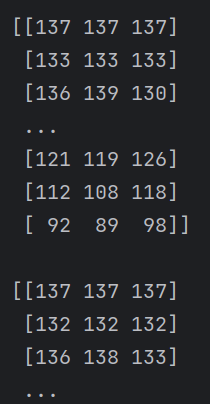
\includegraphics[width=0.15\textwidth]{slike/numpy_frame}
    \captionsetup{font={small}}
    \caption{Ispis dijela vrijednosti za okvir koju vrati $cv::VideoCapture::read$ metoda [autorski rad]}
    \label{fig:ispis_okvira}
\end{figure}

U svakom krugu petlje čita se po jedan okvir i odmah se taj okvir analizira funkcijama $detect\_eyes()$ i $detect\_light()$ kako bi se otkrila pozicija zasljepljujućeg svjetla i očiju (27. i 28. linija koda). Funkcije $detect\_eyes()$ i $detect\_light()$ predstavljaju komponente sustava koje su obrađene u sljedećim poglavljima: "Komponenta za prepoznavanje i pozicioniranje izvora svjetla" i "Komponenta za prepoznavanje i pozicioniranje očiju vozača".

Slika \ref{fig:sustav1} prikaziva kako okviri izgledaju prije otkrivanja zasljepljujućeg svjetla i očiju. Na zaslonu ne trebaju biti otvoreni prikazani prozori sa slike \ref{fig:sustav1}, ali su tu samo kako bi se uvidjelo da sustav odrađiva ono što treba i kako bi se bolje shvatilo kako sustav radi.

\begin{figure}[h!]
    \centering
    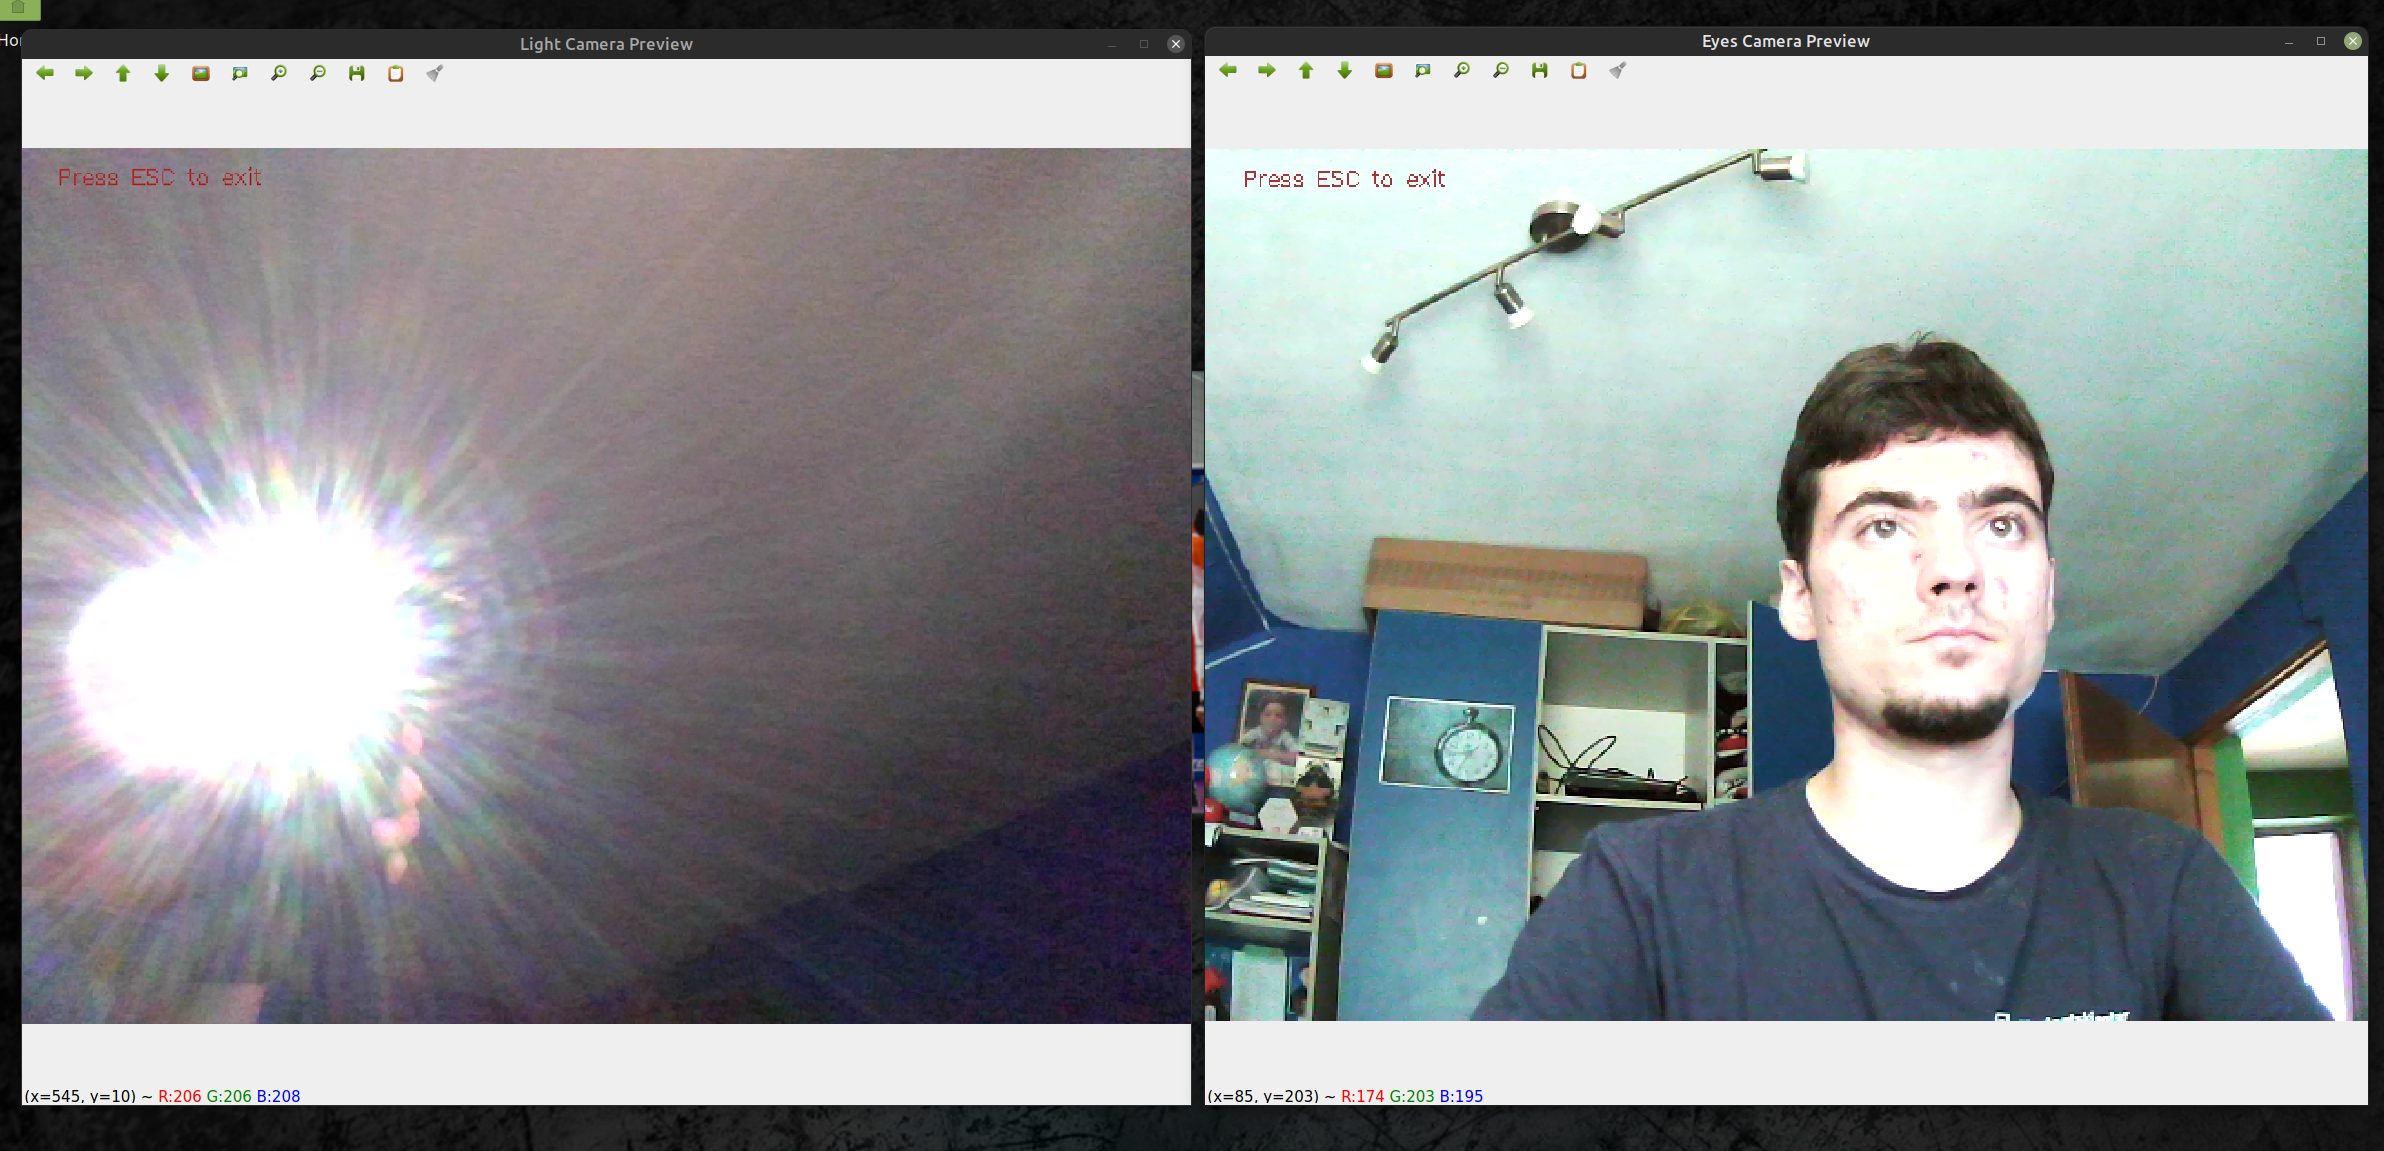
\includegraphics[width=1\textwidth]{slike/sustav1}
    \captionsetup{font={small}}
    \caption{Prikaz okvira prije otkrivanja zasljepljujućeg svjetla i očiju [autorski rad]}
    \label{fig:sustav1}
\end{figure}

\pagebreak
\section{Komponenta za prepoznavanje i pozicioniranje izvora svjetla}

Nakon što se uspješno čitaju okviri s kamere koja gleda okolinu koja je ispred vozača, potrebno je analizirati svaki okvir i otkriti nalazi li se na njima zasljepljujuća svjetlost. Ako se svjetlost nalazi na okviru, potrebno je pronaći točne koordinate svjetlosti na okviru. Ovo poglavlje će kroz programski kod \ref{lst:lstlisting_6} koji prikaziva definiranje funkcije $detect\_light()$ za otkrivanje zasljepljujuće svjetlosti opisati navedeni potrebni zadatak.

\flushleft Potrebno je uključiti biblioteku pomoću sljedećeg programskog koda \ref{lst:lstlisting_numpy}:
\begin{lstlisting}[language=Python, label={lst:lstlisting_numpy}, firstnumber=3, style=colored, caption=Uključivanje biblioteke $numpy$]
import numpy as np
\end{lstlisting}

\begin{lstlisting}[language=Python, label={lst:lstlisting_6}, firstnumber=50, style=colored, caption={Definicija funkcije $detect\_light()$}]
def detect_light(light_frame):
    lower_range = np.array([0, 0, 255])
    upper_range = np.array([240, 11, 255])

    light_hsv_frame = cv.cvtColor(light_frame, cv.COLOR_BGR2HSV)

    color_mask = cv.inRange(light_hsv_frame, lower_range, upper_range)

    contours, _ = cv.findContours(color_mask, cv.RETR_EXTERNAL, cv.CHAIN_APPROX_SIMPLE)

    min_contour_area = 4000
    big_contours = [contour for contour in contours if cv.contourArea(contour) > min_contour_area]

    light_positions = []

    for contour in big_contours:
        light_positions.append(cv.boundingRect(contour))

        x, y, w, h = cv.boundingRect(contour)
        cv.rectangle(light_frame, (x, y), (x + w, y + h), (0, 255, 0), 2)

    light_position_queue.put(light_positions)

    drawText(light_frame, 'Press ESC to exit', (20, 20))

    light_frames_queue.put(light_frame)
\end{lstlisting}

\justifying

Idealno bi bilo kada bi ovakvo rješenje mogli kombinirati i sa senzorom koji može izmjeriti intenzitet svjetlosti jer bi se mogla otkriti i zasljepljujuća svjetlost drugih boja osim raspona bijele boje koji je jedini definiran u ovom rješenju za otkrivanje zasljepljujuće svjetlosti te također bi se svjetlost mogla lakše klasificirati. U programskom kodu \ref{lst:lstlisting_6} definiran je raspon bijele boje koji će se otkrivati na okviru (51. i 52. linija koda). Bijela boja je izabrana zato što je svjetlost najčešće bijele do žute boje.

Kao argument ova funkcija prima okvir koji treba analizirati. Potrebno je tom okviru promijeniti prostor boja (engl. \emph{color space}) iz BGR prostora boja (engl. Blur-Green-Red - BGR; OpenCV koristi BGR prostor boja umjesto RGB prostora boja zbog toga što je prilikom početnih godina OpenCV-a BGR prostor boja bio dosta popularniji kod proizvođača kamera i pružatelja softvera, a tako je i ostalo do danas \cite{Satya}) u HSV prostor boja (54. linija koda) zbog toga što funkcija $inRange()$ biblioteke OpenCV koristi HSV prostor boja te ona će kao argumente primiti HSV okvir i raspon boja. Funkcijom $inRange()$ dobit ćemo masku okvira popunjenu crno-bijelom bojom gdje bijela boja predstavlja objekt od interesa koji se svojom bojom nalazi u definiranom rasponu boje \cite{OpenCV3} (56. linija koda). Na slici \ref{fig:maska} može se vidjeti kako je funkcija $inRange()$ stvorila masku okvira sa crnom i bijelom bojom gdje bijela boja predstavlja zasljepljujuću svjetlost:

\begin{figure}[h!]
    \centering
    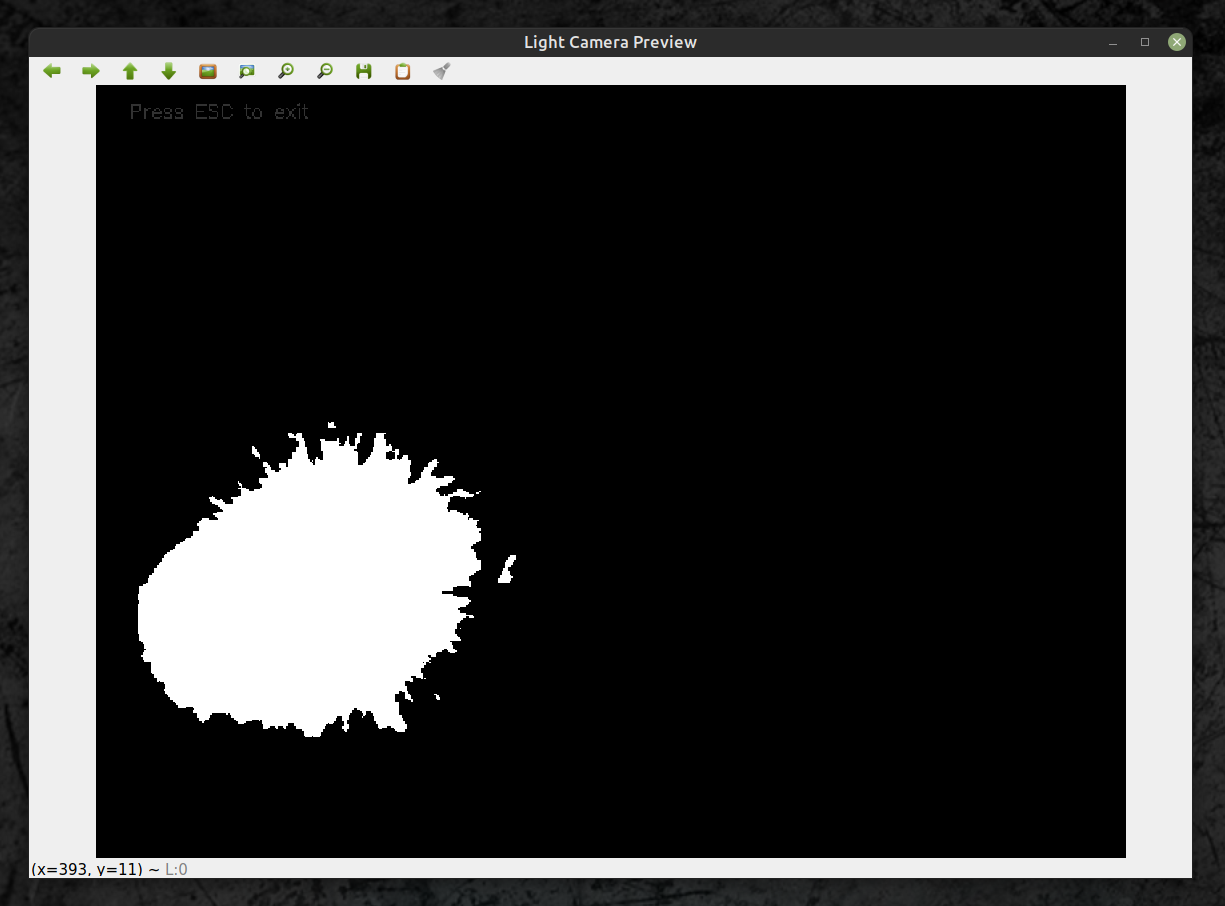
\includegraphics[width=0.6\textwidth]{slike/cb_maska_okvir}
    \captionsetup{font={small}}
    \caption{Prikaz crno-bijele maske okvira [autorski rad]}
    \label{fig:maska}
\end{figure}

Sada se može reći da je zasljepljujuća svjetlost otkrivena, ali se ne zna njezina točna pozicija s koordinatama što će poslužiti kod obavljanja računanja zaštitnog okvira za LCD matricu. Stoga svo ovo provedeno pretvaranje okvira (od originalnog okvira preko pretvaranja u HSV prostor boja do stvaranja crno-bijele maske) je učinjeno zbog toga što će maska okvira biti proslijeđena funkciji $findContours()$ biblioteke OpenCV koja još prima argumente $cv.RETR\_EXTERNAL$ i $cv.CHAIN\_APPROX\_SIMPLE$ koji definiraju kakve će se konture praviti (58. linija koda).

U ovom rješenju kontura predstavlja pravokutnik koji obuhvaća objekt od interesa (bijela boja na slici \ref{fig:maska}) i za taj pravokutnik dobijemo koordinate gornje lijeve točke, visinu i širinu. Funkcija $findContours()$ nije obavezno tražila svo provedeno pretvaranje okvira ali zbog boljeg pronalska kontura preporučeno je da funkcija primi binarni okvir - crno-bijelu masku kako bi rubovi bili što izraženiji \cite{OpenCV4}. Kako bi samo imali konture najizraženijih i najvećih svjetlosti odrađeno je i filtriranje (60. i 61. linija koda).

Sada je potrebno proći kroz svaku pronađenu konturu kako bi ju dodali u $light\_position\_queue$ red i kako bi na originalnom okviru iscrtali zeleni pravokutnik oko zasljepljujuće svjetlosti i spremili originalni okvir u $light\_framesq\_queue$ red (63. do 75. linija koda). Potrebno je naglasiti da pralaleno radi i glavna dretva koja odmah uzima okvire stavljene u red i prikaziva ih u prozorima na zaslonu, a o tome će biti više rijeći u poglavlju "Komponenta za polarizaciju LCD matrice kao reaktivne komponente". Iscrtavanje zelenog pravokutnika na originalnom okviru (slika \ref{fig:sustav2}) napravljeno je samo zbog toga kako bi se uvjerili da otkrivena zasljepljujuće svjetlosti radi.

\begin{figure}[h!]
    \centering
    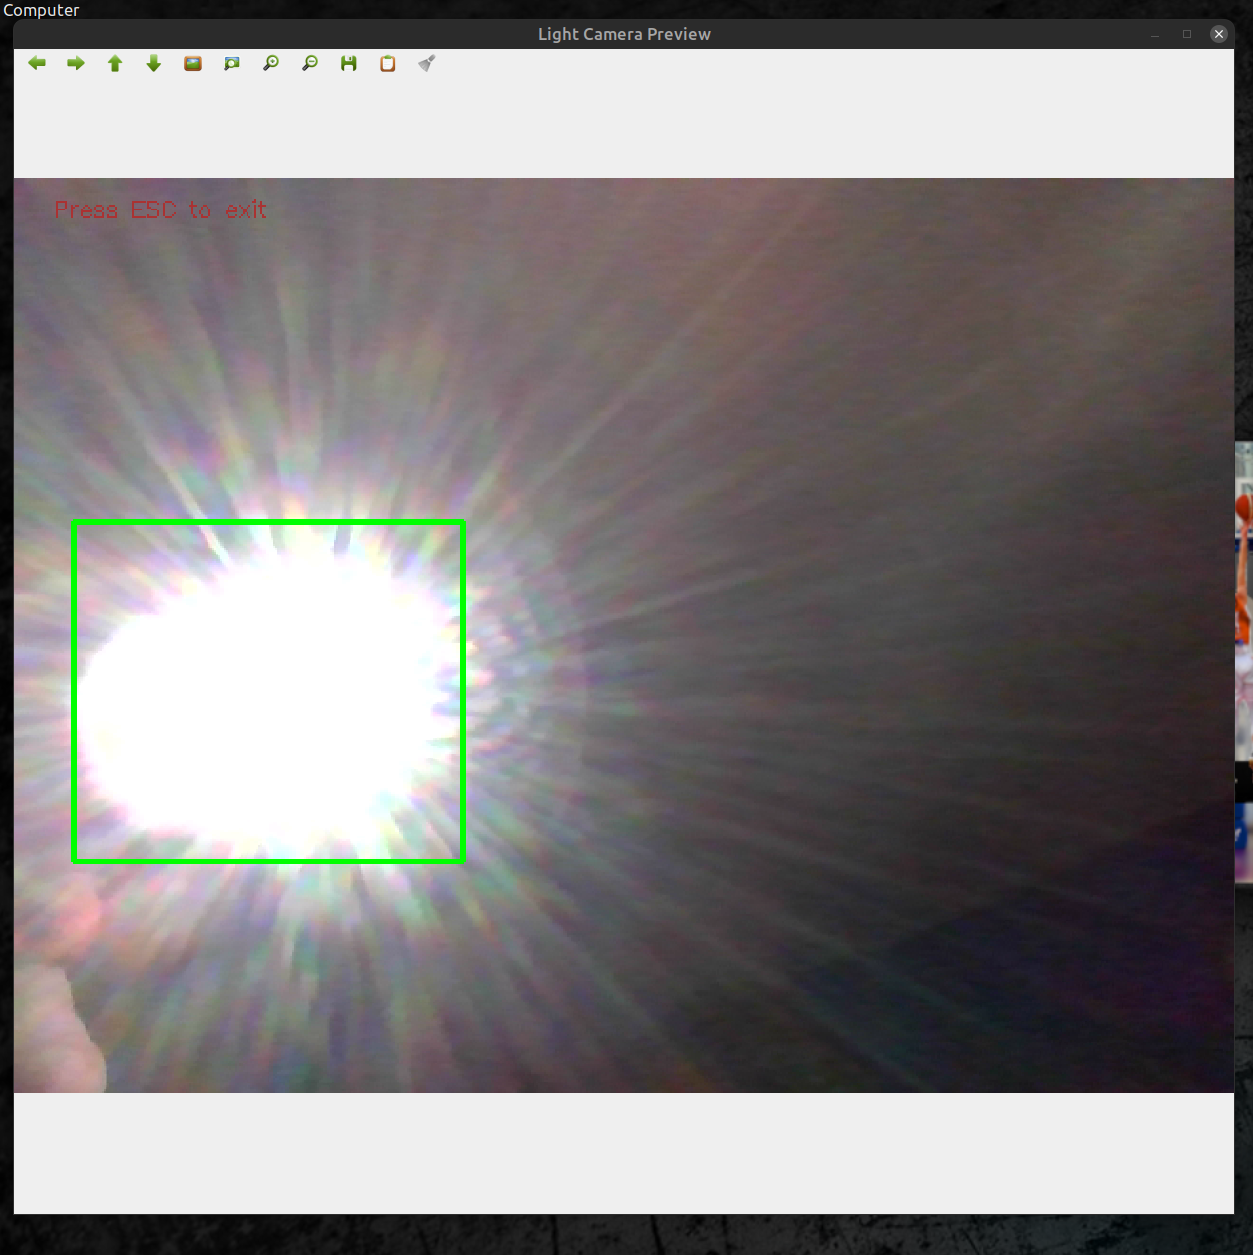
\includegraphics[width=0.4\textwidth]{slike/sustav2}
    \captionsetup{font={small}}
    \caption{Prikaz otkrivene svjetlosti [autorski rad]}
    \label{fig:sustav2}
\end{figure}

\pagebreak
\section{Komponenta za prepoznavanje i pozicioniranje očiju vozača}

Nakon što se uspješno čitaju okviri s kamere koja gleda u vozača, potrebno je analizirati svaki okvir i otkriti nalaze li se na njima oči. Ako se oči nalaze na okviru, potrebno je pronaći točne koordinate očiju na okviru. Ovo poglavlje će kroz programski kod \ref{lst:lstlisting_9} koji prikaziva definiranje funkcije $detect\_eyes()$ za otkrivanje očiju opisati navedeni potrebni zadatak.

\begin{lstlisting}[language=Python, label={lst:lstlisting_9}, firstnumber=33, style=colored, caption={Definicija funkcije $detect\_eyes()$}]
def detect_eyes(eyes_frame):
    eyes_gray_frame = cv.cvtColor(eyes_frame, cv.COLOR_BGR2GRAY)

    eye_cascade_model = cv.CascadeClassifier(cv.data.haarcascades + 'haarcascade_eye.xml')

    eyes = eye_cascade_model.detectMultiScale(eyes_gray_frame, scaleFactor=1.1, minNeighbors=5, minSize=(30, 30))

    eyes_position_queue.put(eyes)

    for (x, y, w, h) in eyes:
        cv.rectangle(eyes_frame, (x, y), (x + w, y + h), (0, 255, 0), 2)

    drawText(eyes_frame, 'Press ESC to exit', (20, 20))

    eyes_frames_queue.put(eyes_frame)
\end{lstlisting}

CascadeClassifier (36. linija koda) je klasa u OpenCV biblioteci koja se koristi za otkrivanje objekata u slikama. Ova klasa implementira algoritam za kaskadnu klasifikaciju koji je temeljen na Haar-like značajkama gdje je je kaskadna funkcija trenirana na mnogo pozitivnih (sadržavaju objekt od interesa) i negativnih fotografija (ne sadržavaju objekt od interesa). \cite{OpenCV5}

Kaskadna klasifikacija je metoda strojnog učenja koja se koristi za otkrivanje objekata u slikama. Ova metoda koristi niz jednostavnih klasifikatora koji su organizirani u kaskadu kako bi brzo i precizno otkrili objekte. Svaki klasifikator u kaskadi analizira sliku i odlučuje je li objekt prisutan ili ne. Ako je objekt prisutan, slika se prosljeđuje sljedećem klasifikatoru u kaskadi, a ako nije, proces se zaustavlja. Haar-like značajke su vrsta značajki koje se koriste u kaskadnoj klasifikaciji. Ove značajke su temeljene na razlici u intenzitetu piksela između susjednih regija slike (Slika \ref{fig:haar_casc}). Haar-like značajke su vrlo jednostavne i brze za izračunavanje, što ih čini idealnima za upotrebu u realnom vremenu za otkrivanje objekata. \cite{KhanTanw2019}

\begin{figure}[h!]
    \centering
    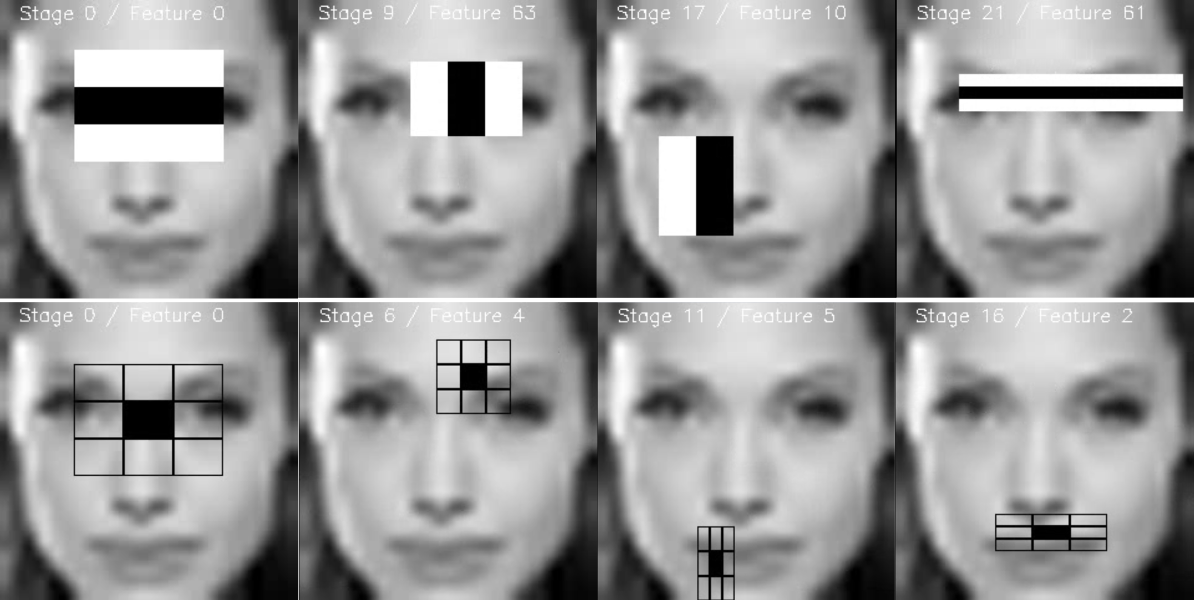
\includegraphics[width=0.6\textwidth]{slike/haar_cascade}
    \captionsetup{font={small}}
    \caption{Prikaz Haar-like značajki \cite{OpenCV-haar}}
    \label{fig:haar_casc}
\end{figure}

\newpage
OpenCV biblioteka sadrži implementaciju CascadeClassifier klase koja omogućuje jednostavnu upotrebu ovog algoritma. Klasa sadrži metode za treniranje i primjenu kaskadnog klasifikatora na slikama. Također omogućuje spremanje i učitavanje prethodno istreniranih klasifikatora. CascadeClassifier se često koristi za otkrivanje lica, tijela i drugih objekata u slikama, a u ovom radu će se koristiti za otkrivanje očiju. Ova metoda je vrlo brza i precizna, što ju čini idealnom za upotrebu u realnom vremenu aplikacijama kao što su video nadzor ili interaktivne igre. \cite{OpenCV5}

Prilikom inicijaliziranja objekta klase $CascadeClassifier$ navodi se što je objekt od interesa - ovdje je to oko (36. linija koda). Kada je objekt inicijaliziran možemo njegovoj metodi $detectMultiScale$ proslijediti okvir (prije nego se krene analizirati okvir, preporučeno je zbog boljih rezultata da se okvir prebaci u sivi prostor boja (34. linija koda) \cite{OpenCV5}.) koji se treba analizirati te je još moguće proslijediti argumenata koji bi utjecali na rezultat. Kao rezultat metoda vraća otkrivene objekte različitih veličina u obliku liste pravokutnika koji opisuju točnu poziciju (koordinate gornjeg lijevog kuta pravokutnika na okviru te njegova duljina i širina) očiju na okviru \cite{OpenCV6}. Lista pravokutnika se sprema u $eyes\_position\_queue$ red za daljno računanje (40. linija koda), a još će se i lista pravokutnika iscrtati na originalnim okvirima i spremiti u $eyes\_frames\_queue$ red kako bi prilikom prikazivanja okvira uvidjeli da komponenta pravilno radi (slika \ref{fig:sustav3}).

\begin{figure}[h!]
    \centering
    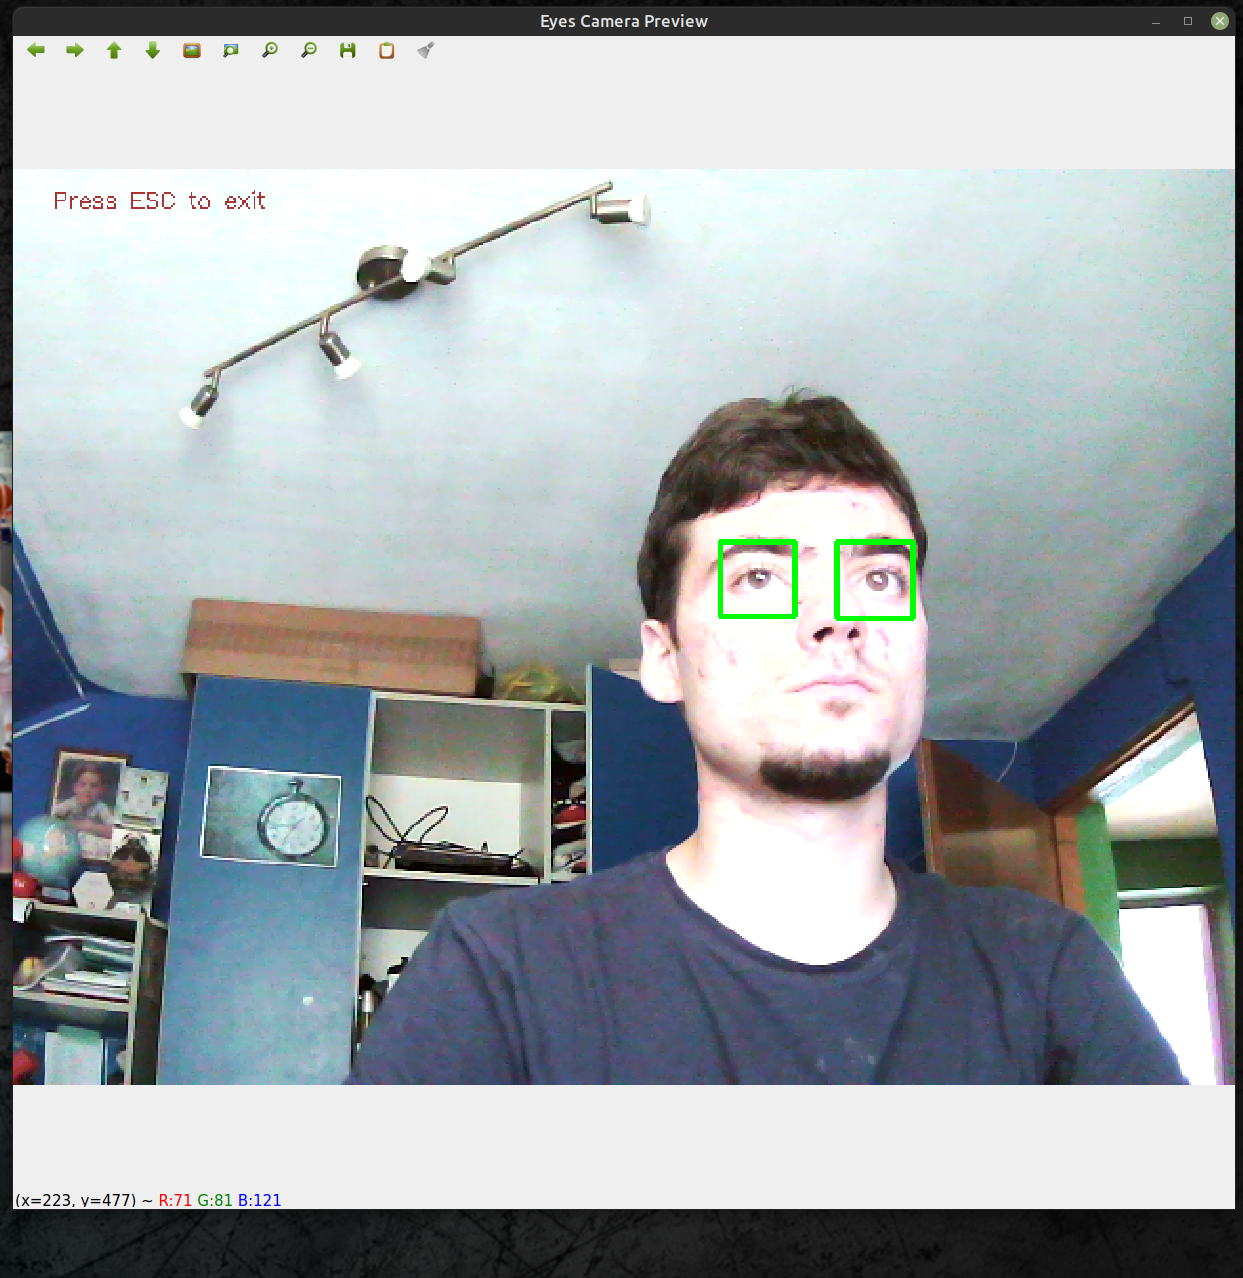
\includegraphics[width=0.4\textwidth]{slike/sustav3}
    \captionsetup{font={small}}
    \caption{Prikaz otkrivenih očiju [autorski rad]}
    \label{fig:sustav3}
\end{figure}

\pagebreak
\section{Komponenta za polarizaciju LCD matrice kao reaktivne komponente}

Kada su pozicije zasljepljujućeg svjetla (crveni okvir na Slici \ref{fig:sustav6}) i očiju (zeleni okvir na Slici \ref{fig:sustav6}) poznate, potrebno je izračunati na kojem mjestu treba zatamniti LCD matricu, a selektivno zatamnjivanje matrice ustvari znači postavljanje na crnu boju jednog dijela novog zaštitnog okvira (crni okvir na Slici \ref{fig:sustav6}) koji će se prikazivati u prozoru na LCD matrici. Kako bi se bolje shvatila problematika, sljedeća slika \ref{fig:sustav6} prikazuju pojednostavljen prikaz sustava u trodimenzionalnom koordinatnom sustavu sa jednakom udaljenošću od matrice.

\begin{figure}[h!]
    \centering
    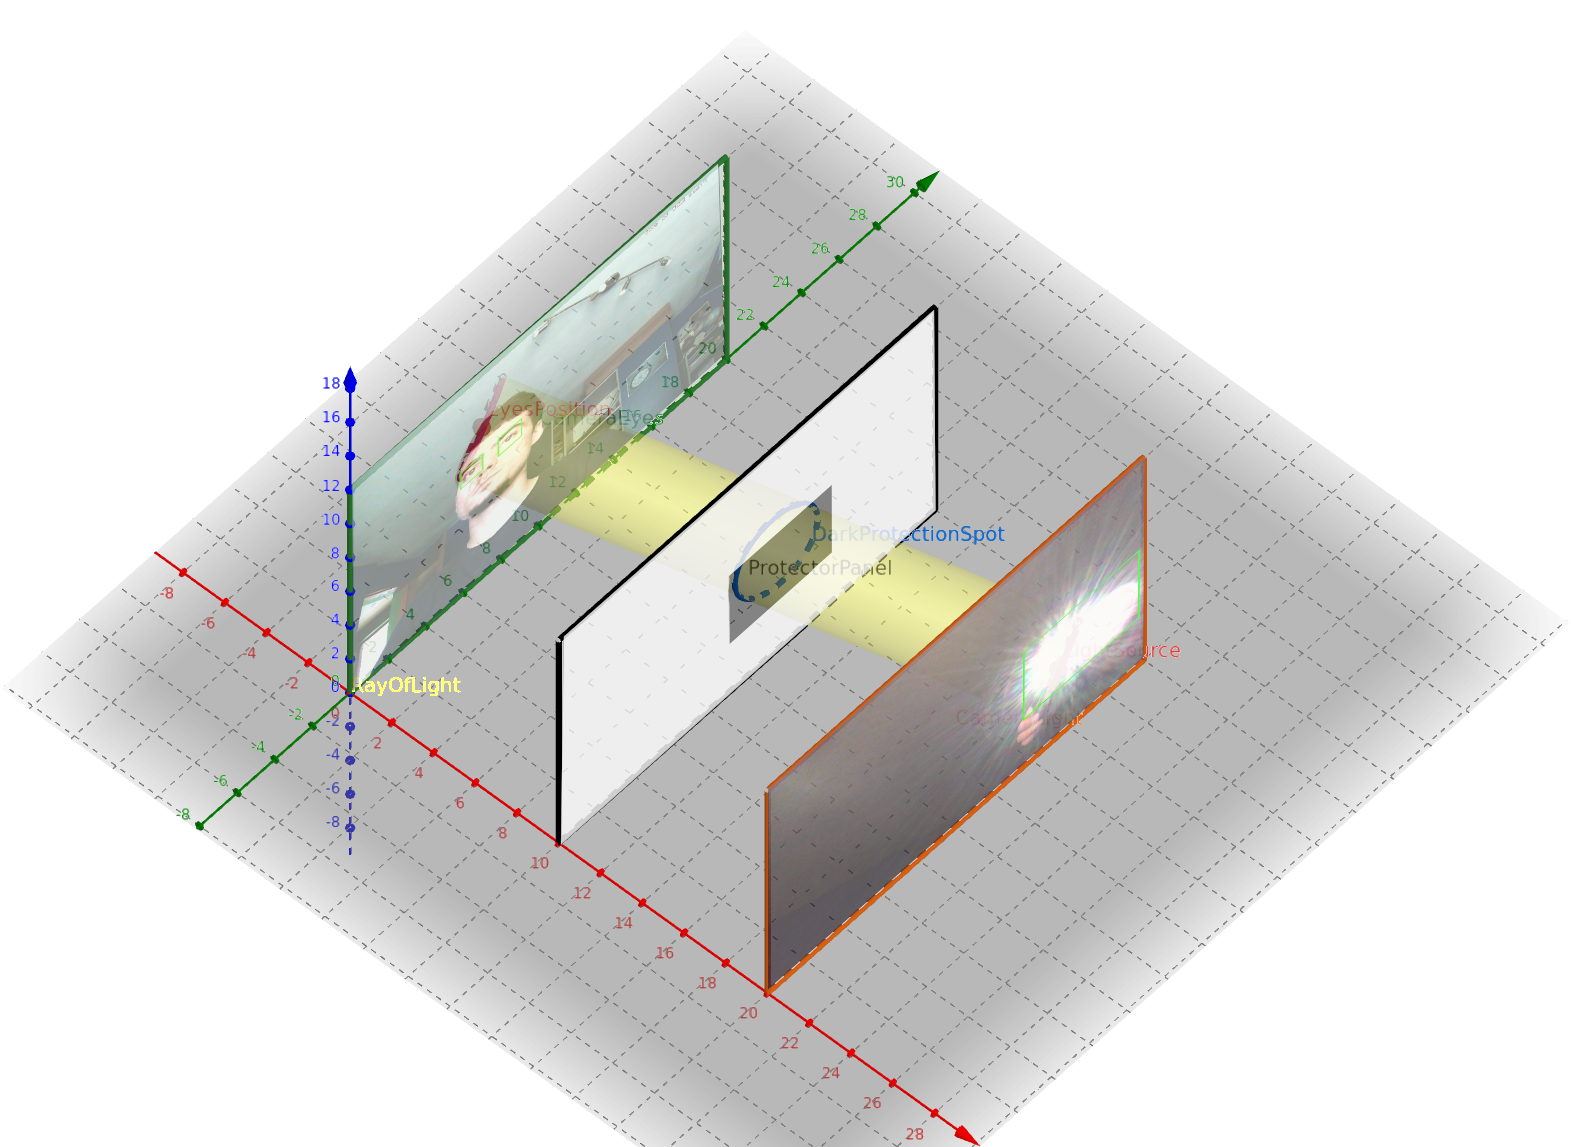
\includegraphics[width=0.8\textwidth]{slike/sustav6}
    \captionsetup{font={small}}
    \caption{Pojednostavljen prikaz sustava sa simbolično prikazanim okvirima u trodimenzionalnom koordinatnom sustavu sa jednakom udaljenosti od matrice [autorski rad]}
    \label{fig:sustav6}
\end{figure}

Zbog jednostavnosti izračuna, zamišljena udaljenost vozača od LCD matrice i udaljenost zasljepljujućeg svjetla od LCD matrice uzeta je kao jednaka. Shodno tome, sljedeća slika \ref{fig:sustav4} prikaziva kako ovaj graf izgleda iz druge perspektive, odnosno u dvodimenzionalnom koordinatnom sustavu.

\begin{figure}[h!]
    \centering
    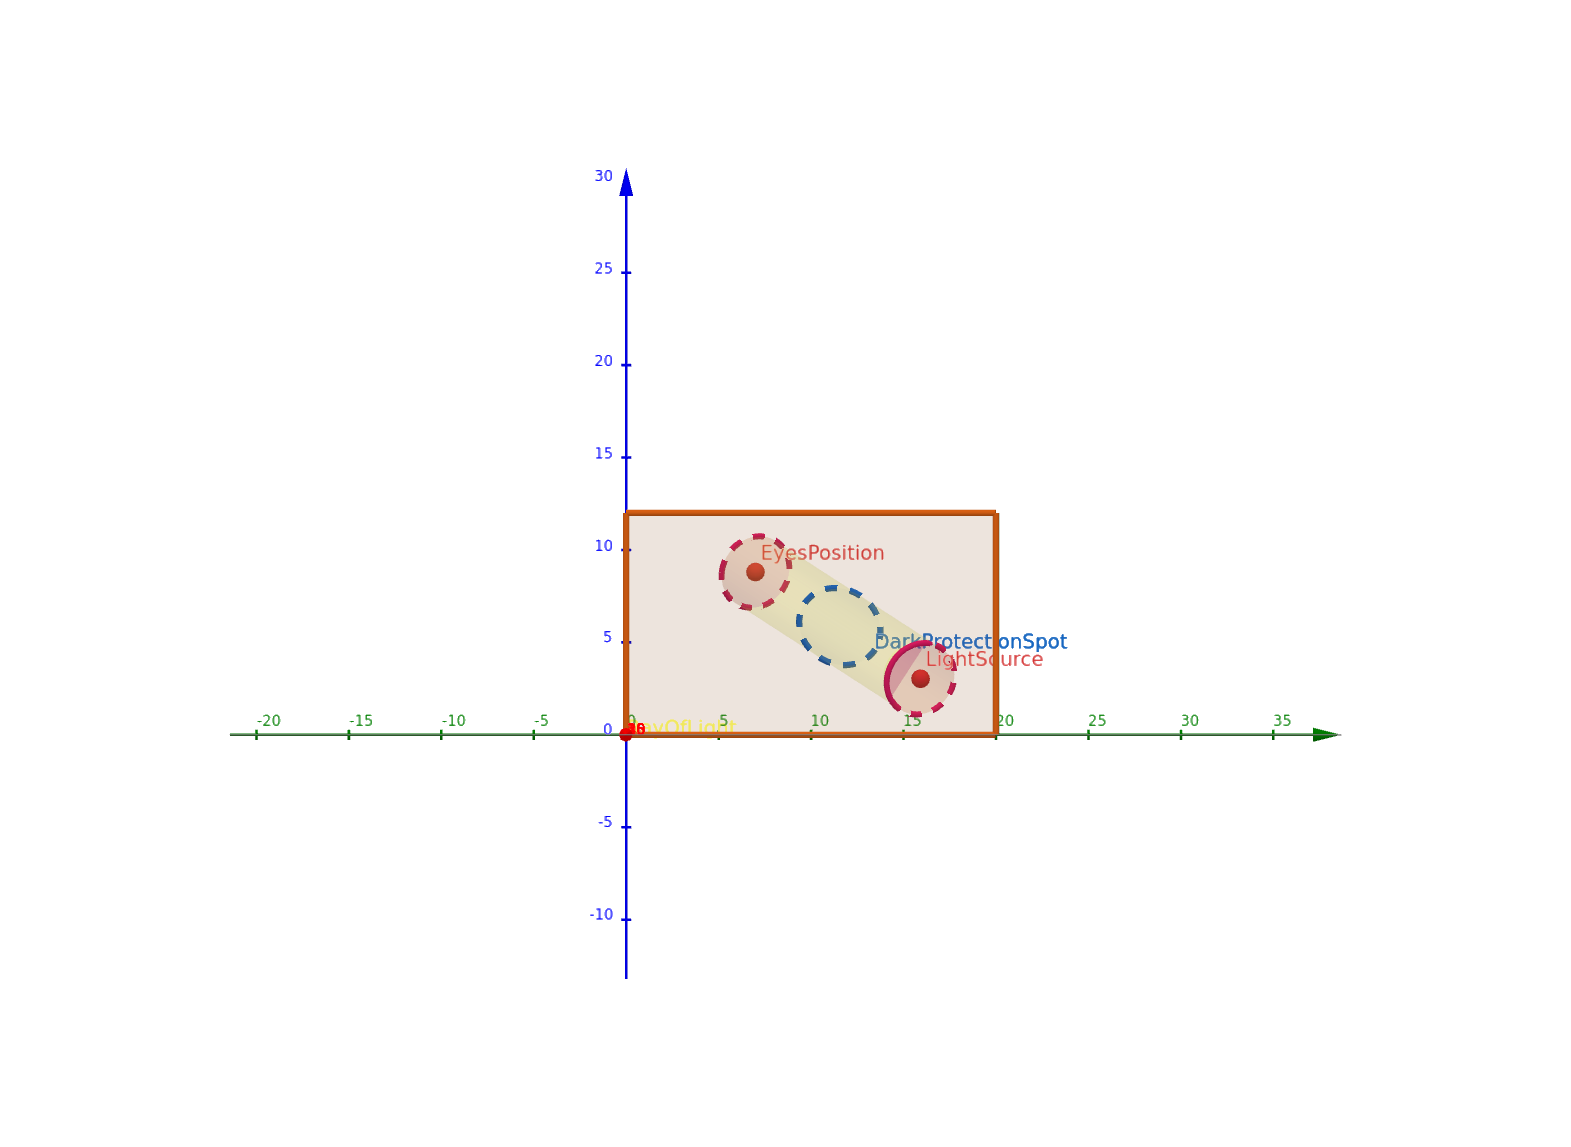
\includegraphics[width=0.8\textwidth]{slike/sustav4}
    \captionsetup{font={small}}
    \caption{Pojednostavljen prikaz sustava u dvodimenzionalnom koordinatnom sustavu [autorski rad]}
    \label{fig:sustav4}
\end{figure}

\newpage
Nakon razmatranja slike \ref{fig:sustav4} sustava u dvodimenzionalnom polju, dolazi se do zaključka da bi se pozicija pravokutnika crne boje koji će sprječavati svjetlosni snop na zaštitnom okviru mogao nalaziti na polovištu dužine između pozicije očiju i pozicije svjetlosti, što je urađeno programskim kodom \ref{lst:lstlisting_10}.

\begin{lstlisting}[language=Python, label={lst:lstlisting_10}, firstnumber=33, style=colored, caption={Definicija funkcije $create\_protection\_frame()$}]
def create_protection_frame():
    frame_width = 640
    frame_height = 480

    protection_frame = np.ones((frame_height, frame_width, 3), dtype=np.uint8) * 255

    eye_positions = eyes_position_queue.get()
    light_positions = light_position_queue.get()

    for light_position in light_positions:
        for eye_position in eye_positions:
            eye_x, eye_y, eye_w, eye_h = eye_position
            light_x, light_y, light_w, light_h = light_position

            protection_x = (eye_x + light_x) // 2

            protection_y = (eye_y + light_y) // 2

            cv.rectangle(
                protection_frame,
                (protection_x, protection_y),
                (protection_x + light_w, protection_y + light_h),
                (0, 0, 0),
                -1
            )

    eyes_position_queue.task_done()
    light_position_queue.task_done()

    return protection_frame
\end{lstlisting}

Prikaz funkcioniranja sustava - link na video: \href{https://foi-my.sharepoint.com/:v:/g/personal/spetrovic20_foi_hr/ERfsxYop3VFCnwyEWHfwgokB6hWikBInY5lpKwYVjjt91A?nav=eyJyZWZlcnJhbEluZm8iOnsicmVmZXJyYWxBcHAiOiJPbmVEcml2ZUZvckJ1c2luZXNzIiwicmVmZXJyYWxBcHBQbGF0Zm9ybSI6IldlYiIsInJlZmVycmFsTW9kZSI6InZpZXciLCJyZWZlcnJhbFZpZXciOiJNeUZpbGVzTGlua0RpcmVjdCJ9fQ&e=REgtGV}{https://foi-my.sharepoint.com}

\section{Testiranje sustava}

\pagebreak
\chapter{Zaključak}

Ovdje treba sažeto rezimirati najvažnije rezultate razrade teme rada. Potrebno je sažeto opisati što je predmet rada, koje su metode, tehnike, programski alati ili aplikacije korištene u razradi rada te koje su pretpostavke dokazane, a koje opovrgnute. Sadržajno, ono što se u uvodu rada najavljuje i kasnije je obuhvaćeno u samom radu, moralo bi biti opisano u zaključnom dijelu kroz rezultate rada.

\printbibliography[title=Popis literature]
\addcontentsline{toc}{chapter}{Popis literature}

\listoffigures
\addcontentsline{toc}{chapter}{Popis slika}

\lstlistoflistings
\addcontentsline{toc}{chapter}{Popis programskih kodova}

\end{document}
